%%
%%  chapter05.tex - Obstacle Detection and Planning for Autonomous Vehicles based on Computer Vision Techniques
%%
%%  Copyright 2014 Néstor Morales <nestor@isaatc.ull.es>
%%
%%  This work is licensed under a Creative Commons Attribution 4.0 International License.
%%

\graphicspath{{./images/chapter05/bmps/}{./images/chapter05/vects/}{./images/chapter05/}}

\chapter{3D object tracking}\label{ch:chapter05}

As we have seen in previous chapters, we still have not solved completely the problem of detection and tracking of the obstacles. Image comparison could be, as said, a good input point for an obstacle classifier, but it is still not able to locate obstacles in the real world with respect to a map o to the vehicle. Also, it is not able to track the obstacles and it is very dependent on the goodness of the database of the area in which the vehicle is driving. Non-rigid point set registration method is not able to detect obstacles using moving cameras. \notsure{Stixels can be a solution, but they do not consider obstacles further from a first plane and they assume a flat road}. 

In this chapter, we will describe a method that, using a point cloud generated from a pair of moving stereo cameras, is able to detect obstacles and model them as a set of voxels. Also, it is able to decide the direction in which objects are moving to. The method described here is inspired in the work by \cite{danescu2012particle}, in the way that a particle filter is used over an occupancy grid in order to detect the obstacles and their directions. However, this method uses a two-dimensional grid. As said in section \ref{ch:chapter00_02_05}, methods based on such a grid are related to which we named as 2.5D methods. The main disadvantages of this kind of methods is that they consider all the obstacles as lying in the ground, and are represented as a convex cuboid that doesn't take into account the complexities of certain obstacles.
As commented in previous sections, Verdino is thought to work in crowded areas, like pedestrian streets or touristic complexes, in which an overestimation of the size of obstacles can lead to an inefficient behavior. So we decided to extend the original method of \cite{danescu2012particle} in order to make it fully three-dimensional, by using a voxelized grid instead of the original cartesian/polar grid, and including some improvements in order to reduce the number of fake positives, among others.

\section{The Method}\label{ch:chapter05_01}

In this method, we generate a voxelized occupancy grid in which the world surrounding the vehicle is divided into a discrete number of voxels of the same size. For each voxel, a occupancy probability is assigned based on the number of points inside the volume represented by it and its neighborhood. Also, during the process, a set of particles will be assigned dynamically during the execution, based on a 3D generalization of the weighting and resampling mechanism described in \cite{isard1998condensation}. These particles will have a double function:
\begin{enumerate}
 \item Denoting hypotheses (as happens with classical particle filters).
 \item Being the building blocks of our world model.
\end{enumerate}

Like this, at each frame, the set of particles obtained in the previous frame (each of these with a certain pose ${(x, y, z)}$ and speed ${(vx, vy, vz)}$) will be evolved using their movement model and assigned to the corresponding voxel, attending to the time that passed between frames and the ego-motion. Then, these particles are re-weighted and resampled.

At this point, particles that passed the resampling process are used to construct the objects that model the environment, joining all these voxels that share a similar orientation and speed. This object reconstruction is done by using a flood fill approach, in a way quite similar to that described in \cite{broggi2013}, but using the vectors of each voxel, instead of color information, as done in their work.

This particle-based approach inherits some advantages from the previous work by \cite{danescu2012particle}:
\begin{itemize}
 \item \emph{It is not necessary to estimate the probability distribution of the speed or the orientation.} These distributions, which in the past have been approximated as histograms (\cite{chen2006dynamic}), Gaussian mixtures (\cite{gindele2009bayesian}) or higher dimensions (\cite{coue2006bayesian}), are not required anymore due to the use the particles. This distribution is obtained directly from the surviving particles of each voxel. 
 \item \emph{Easy encoding of the past and present knowledge from sensor data.} The usage of a voxel grid makes this easier, and allows updating it dynamically when new information is available with a little computational cost.
\end{itemize}

Also, we add some new advantages in our approach:
\begin{itemize}
 \item \emph{Hierarchical object pose, orientation and speed detection.} Object units are detected at lower level as individual voxels, for which we know their individual speed and pose. Joining all these voxels together, we obtain the whole obstacle, whose pose and speed is directly dependent on the voxels which compose it. 
 \item \emph{Fully 3D perception of the object detected.} No previous assumption of the shape of the obstacles is taken, providing an accurate estimation of complex obstacles. The usage of voxels instead of cuboids, allows to have a clear idea of the actual shape of an obstacle, avoiding the overestimation of their real size, which is not acceptable for an application like that described in this Thesis. In this sense, we can have an accurate idea of 3D boundaries of an obstacle or reject it in case it is hanging, like in the case of traffic lights.
 \item \emph{No color information is used.} As we do not use color information coming from the input 3D point cloud, our implementation is ready to accept data from other sensors different from a stereo pair, like \ac{LIDAR}.
 \item \emph{Collaborative update of the grid.} The usage of a voxel grid also allows combining several input sources at the same time. We have not done any work in this sense, but our implementation is ready for such application.
\end{itemize}

The method pipeline is based on six different steps, depicted in figure \todo{ \ref{fig:cp05_pipeline_general} }:
\begin{enumerate}
 \item \emph{3D point cloud generation.} As said before, our implementation is able to work from data coming from any kind of sensor, but in this work, we have been working with stereo cameras. In this step we obtain, from a pair of calibrated images provided by a stereo pair of cameras, a set of 3D points that will be the actual input for our algorithm. At implementation level, this process is done in a separate process, so the point cloud can be used for other tasks in the system. More details of this process are given at section \todo{ \ref{chapter05_01_01} }.
 \item \emph{Ego-motion.} By using images, the orientation and speeds computed for the different objects is biased by the speed of the own vehicle. To avoid this, we need to know our own movement. In section \todo{ \ref{chapter05_01_02} }, this process is better explained.
 \item \emph{Voxelization.} Each of the 3D points obtained in the first step is assigned to a certain voxel. Each voxel has a certain resolution, which covers a parameterized section of the world. In our tests, we have used voxels of a resolution of $(0.25x0.25x0.25)$\,m in the $X$, $Y$ and $Z$ dimensions, respectively, covering a volume going from $-4$\,m to $+4$\,m in the $X$ axis; $0$ to $+24$\,m in the $Y$ axis; and $0$\,m to $3.5$\,m in the $Z$ axis. This process, and how probabilities are assigned to each voxel is explained at section \todo{\ref{chapter05_01_03}}.
 \item \emph{Voxel pose and speed computation.} Based on a \ac{PF} and in the probabilities assigned in the previous step, we calculate the pose and speed of each of the voxels in the grid, as explained in section \todo{\ref{chapter05_01_04}}.
 \item \emph{Object reconstruction.} Once we know the pose and speed of each voxel, and based on a flood fill procedure inspired in the work by \cite{broggi2013} and in the vectors already obtained, similar voxels are assigned to a common final obstacle. For each segmented object, orientation and speed is computed based on the vectors belonging to each of the associated voxels (See section \todo{\ref{chapter05_01_05}}).
 \item \emph{Planning and obstacle avoidance.} Once we know the exact position of the vehicles, and their future movement, we can integrate the results into the rest of the system and use it for the calculation of safe and smooth paths. This process will be described in more depth in the following chapters, in sections \todo{ \ref{chapter05_01_06} }.
\end{enumerate}

\begin{figure}[thb]\label{fig:cp05_pipeline_general}
  \centering
  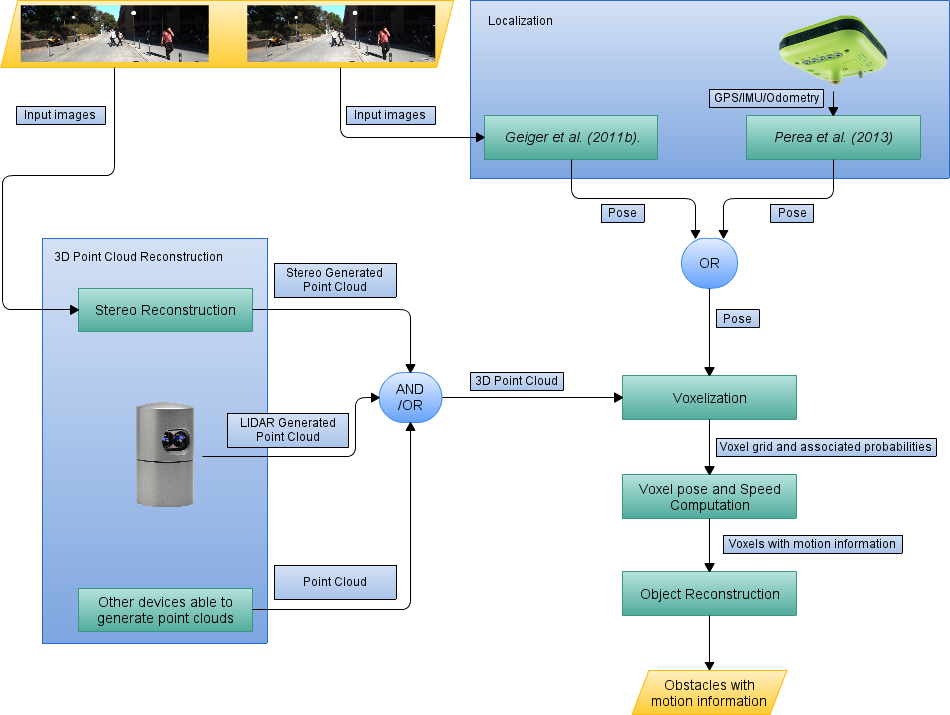
\includegraphics{pipeline_general}
  \caption{Pipeline of the different steps of the method. \todo{Me olvidé de poner el módulo encargado de filtrar los puntos antes de la fase de voxelizado} }
\end{figure}

In the following sections, all these steps will be explained in a bigger detail.

\subsection{3D point cloud generation}\label{ch:chapter05_01_01}

In this stage, a pair of calibrated images is received and transformed into a disparity map, that will allow us to get the corresponding 3D point cloud. In \todoref{XXX}, we evaluated a set of algorithms, including some pre- and post-processing filters, in order to know which of these is the most suitable for outdoor autonomous navigation applications. From this evaluation, we concluded that best results were given by the configuration we named as \emph{Census-SGM Conf 2}. Unfortunately, we had not access to the optimized version of this configuration at the moment of developing the method explained in this chapter. In the other hand, in the same comparison, we saw that both \emph{BT-SGM} and \emph{ELAS} algorithms had also a good response, and we had an implementation of both of them. The question is: what is the most suitable algorithm for our approach? 

In section \ref{ch:chapter05_02_01}, a comparison between both \emph{BT-SGM} and \emph{ELAS} algorithms is performed. After this evaluation, we concluded that both because some quality reasons, as the average error shown in the \ac{LGT} tests in chapter \todoref{XXX-algs-eval}; and due to performance reasons, as shown in the chart at \todoref{XXX-ELAS_BTSGM_times}, ELAS is the most suitable algorithm for the method presented in this chapter.

In figure \ref{fig:cp05_full_filtered_pointcloud}, we can observe the relation between the point cloud generated and the coordinates frame located in the center of the left camera. In this coordinate system, $X$ axis is pointing to the right, $Y$ is the depth of the scene, and $Z$ the height. The rest of frames are explained in more detail in section \todoref{XXX}.

\begin{figure*}[t]
        \centering
        \begin{subfigure}[b]{0.475\textwidth}
                \centering
                \caption{Full Point Cloud}
                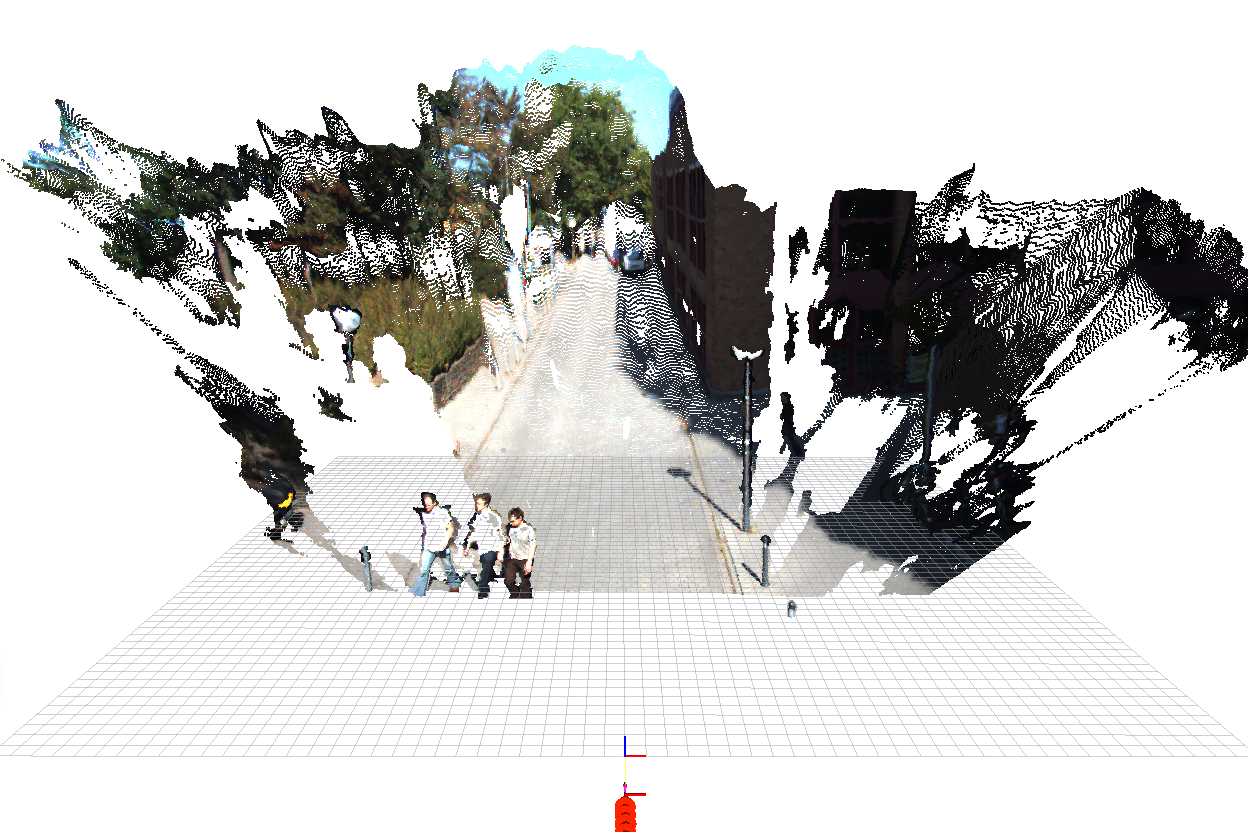
\includegraphics[width=\textwidth]{fullPointCloud}\label{fig:cp05_full_pointcloud}
        \end{subfigure}%        
        ~ 
        \begin{subfigure}[b]{0.475\textwidth}
                \centering
                \caption{Filtered Point Cloud}
                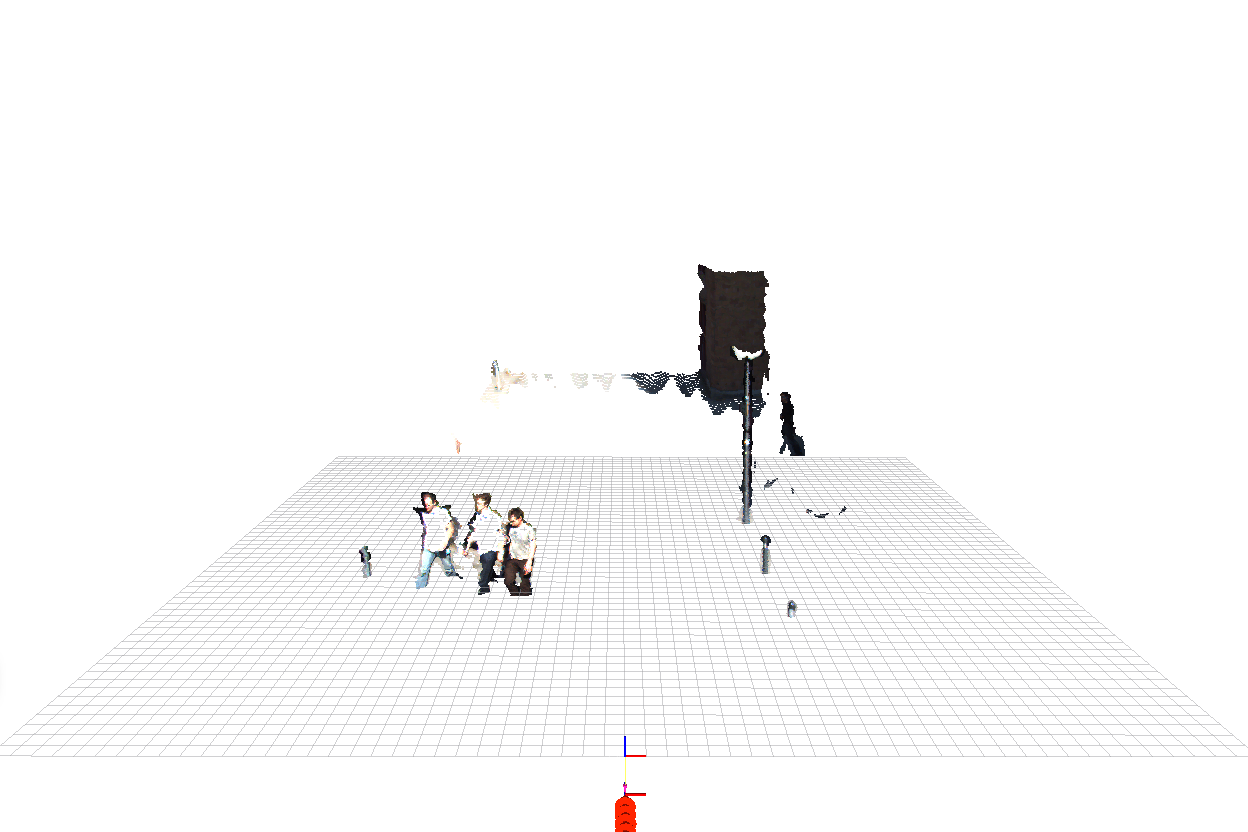
\includegraphics[width=\textwidth]{filteredPointCloud}\label{fig:cp05_filtered_pointcloud}                
        \end{subfigure}%
        \caption{Comparison of a point cloud obtained using \emph{ELAS}, before and after the filtering.}\label{fig:cp05_full_filtered_pointcloud}
\end{figure*}

\subsubsection{Point cloud filtering}\label{ch:chapter05_01_01_01}

Once we have obtained the point cloud, we segment the salient volumes by assuming a flat ground. We remove the points below a plane defined by $XY$, as well as those points that are too far from the origin centered at the left camera to fall inside the voxel grid. This distance, and the resolution of each voxel, is parameterized for each dimension, and determines the size of the grid, so

\begin{equation}\label{eq:cp05_filter_limits}
\begin{cases}
W = (I_{max}(X) - I_{min}(X)) / {DX} \\
L = (I_{max}(Y) - I_{min}(Y)) / {DY} \\
H = (I_{max}(Z) - I_{min}(Z)) / {DZ}
\end{cases}
\end{equation}

Here, $W$, $L$ and $H$ are the width, length and height of the voxel grid. $DX$, $DY$ and $DZ$, are the parameterized resolutions of each voxel at dimensions $X$, $Y$ and $Z$, respectively. $I_{max}(d)$ and $I_{max}(d)$ represent the maximal and minimal value of the interval taken in consideration at each dimension $d$. As depicted in the diagram at figure \ref{fig:cp05_intervals}, the left camera is in the center of the grid in the $X$ and $Z$ dimensions, and at the minimal depth in the other dimension.

\begin{figure*}[t]
        \centering
        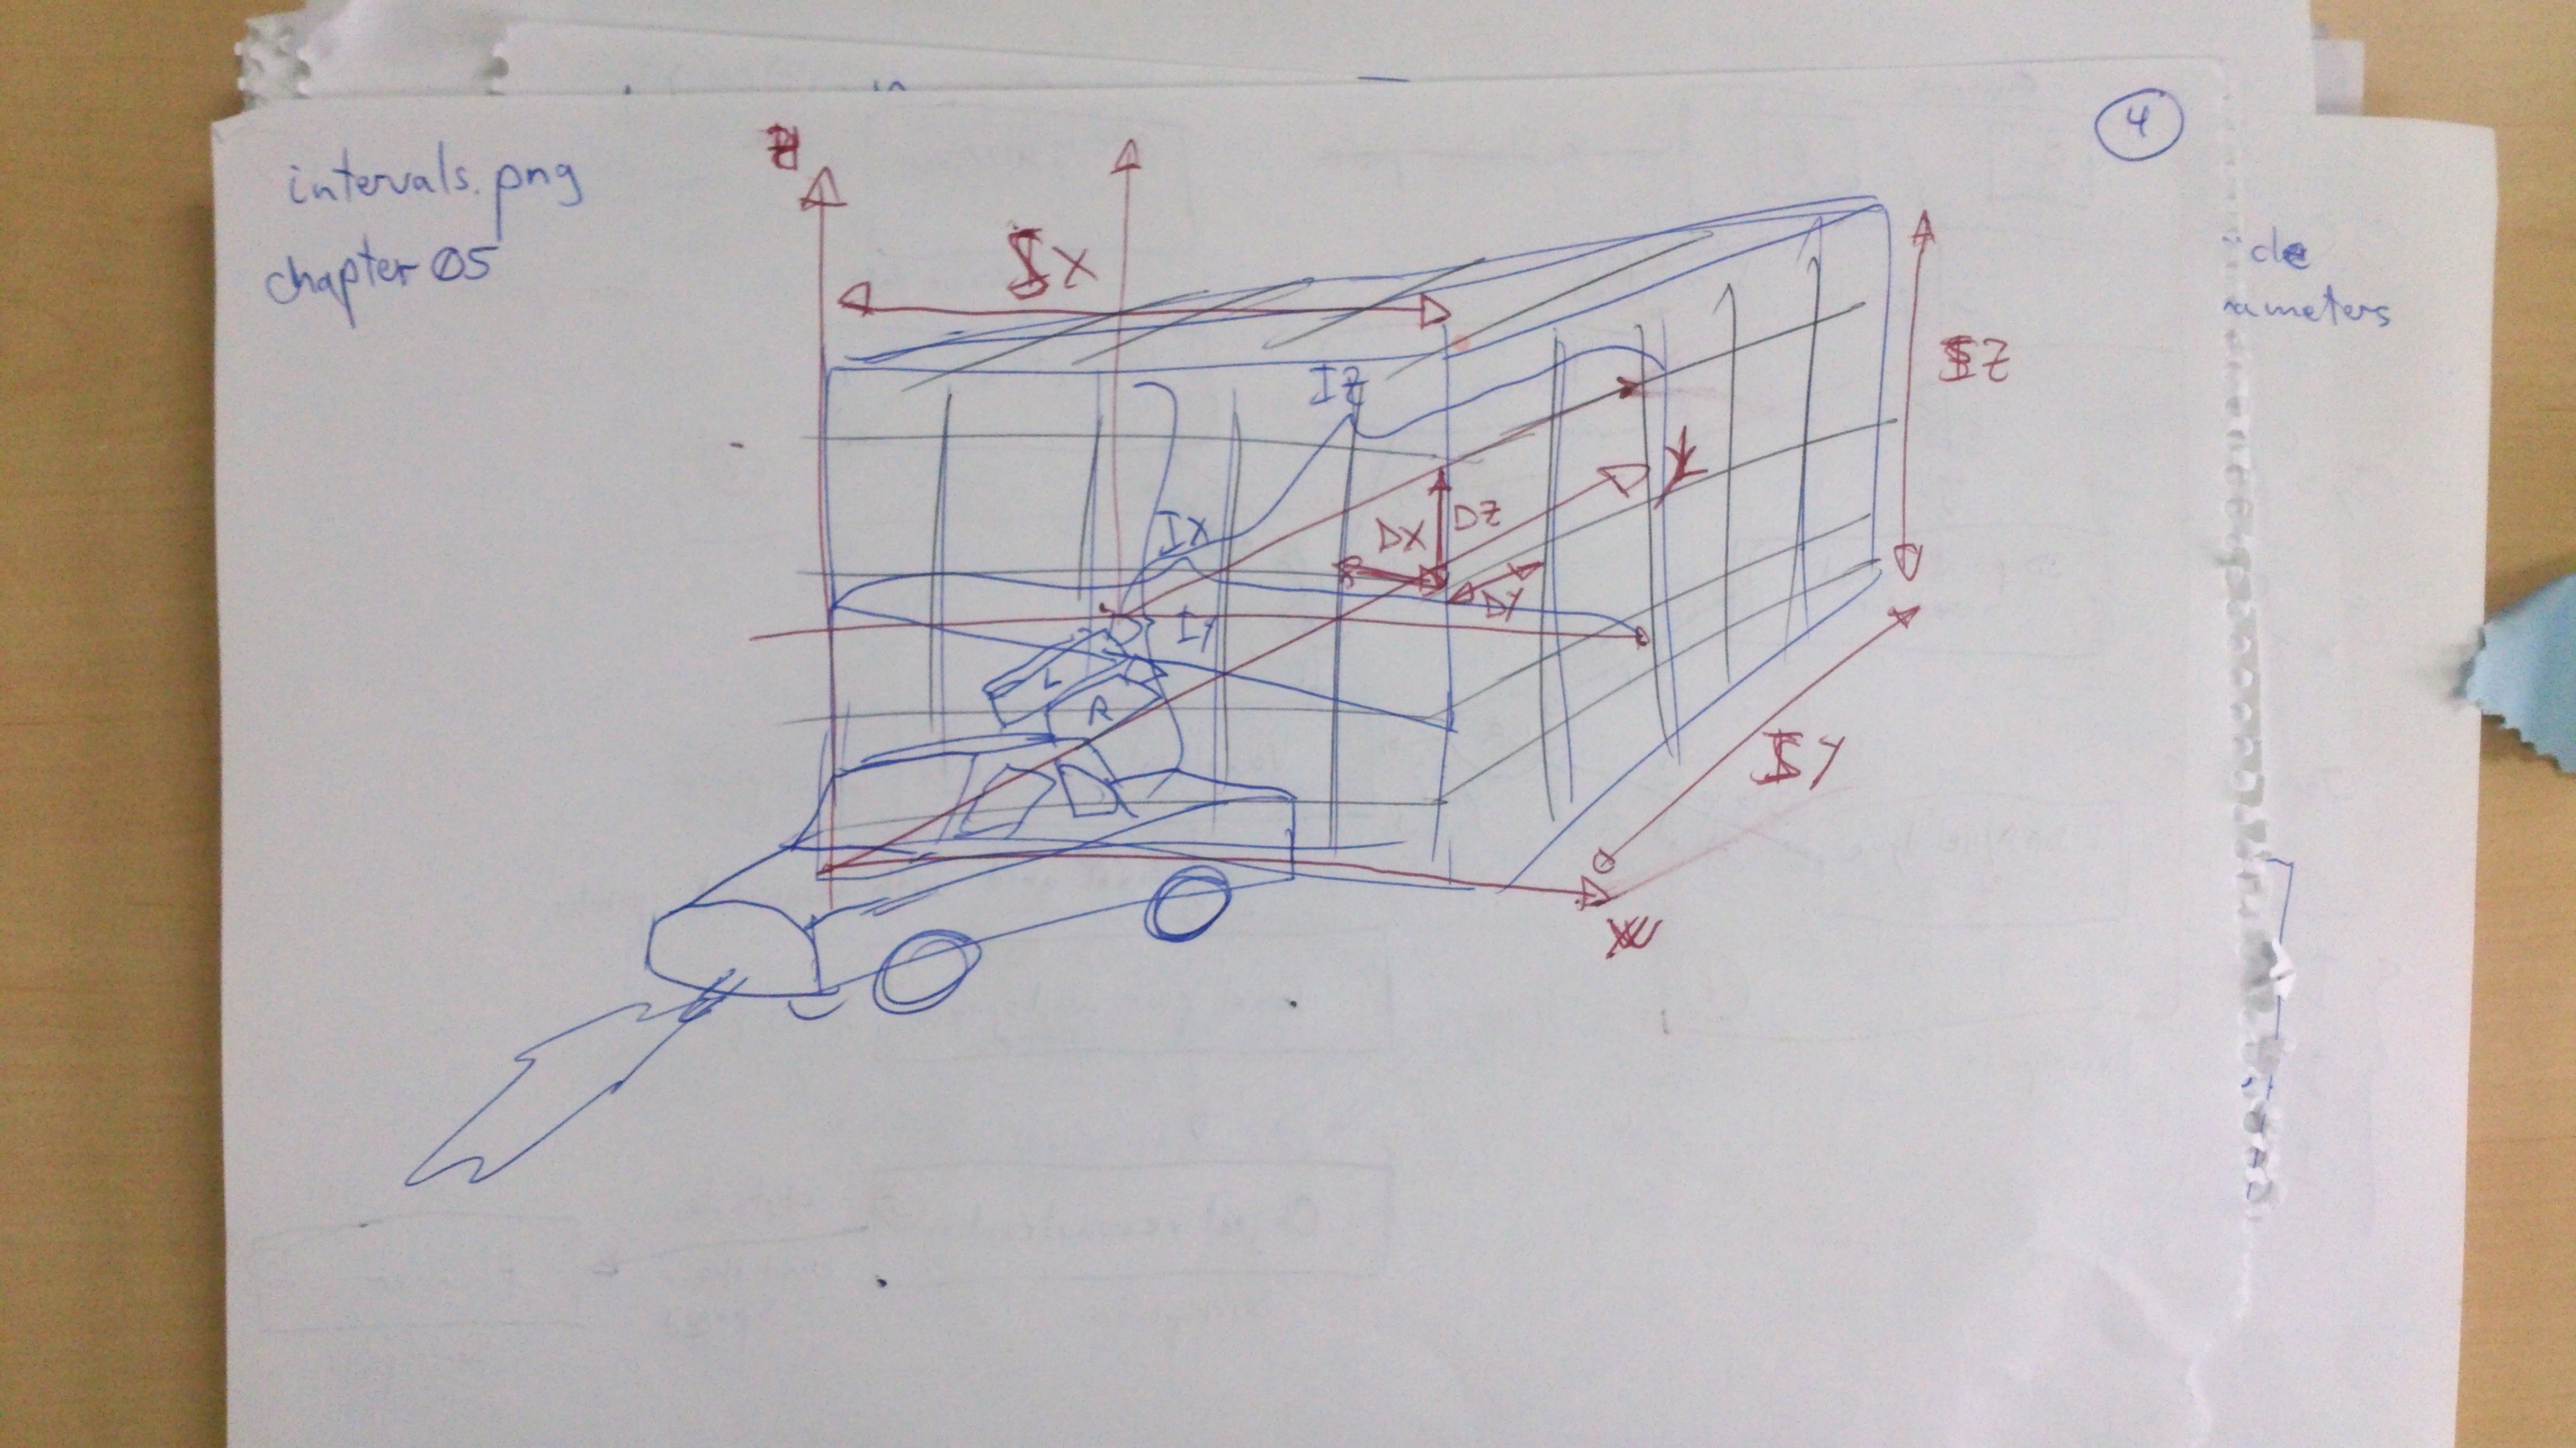
\includegraphics[width=\textwidth]{intervals}
        \caption{Representation of how the voxel grid is computed. Graphical representation of $\{X, Y, Z\}$, $\{DX, DY, DZ\}$, $\{W, L, H\}$ and $\{(I_{min}(n), I_{max}(n))  | n \in \{X, Y, Z\}\}$ are included, for the sake of clarity.}\label{fig:cp05_intervals}
\end{figure*}

At the end of this process, we will have the filtered point cloud $\mathcal{P}$, which will be the input for the 3D reconstruction stage.

\subsubsection{Using other sensors}\label{ch:chapter05_01_01_02}

Despite we have oriented this work to the usage of a stereo camera as input device, the point cloud generation step and filter step have been implemented as separate processes and, as we will see later, no color information is used. So other sources providing a 3D point cloud stream are acceptable for our algorithm. Also several sensors can provide data simultaneously.

\subsection{Ego-motion}\label{ch:chapter05_01_02}

By using a point cloud referred to the left camera (or a given sensor), speeds and orientations are biased by the movement performed by the ego-vehicle between frames. This movement must be compensated, so we need to know the ego-motion performed by the vehicle. This can be done, in one hand, using the localization method used by Verdino (\cite{Perea2013mcl}), based on the information obtained from an odometric sensor, which combined with the \ac{GPS} signal and an \ac{IMU} device, gives a precise localization Other way to do this is by using a visual odometry system, like that proposed by \cite{geiger2011stereoscan}. In section \todoref{XXX}, a comparison between a sensor-based odometric system and a image-based odometry system is performed, concluding that both approaches can be used indistintly without affecting to the results of our method. As some datasets does not include this odometry information, we have decided to use the visual odometry method in our evaluation tests.

In figure \ref{fig:cp05_tfs}, we can see the different positions at which the vehicle has been located at previous frames, as well as the rest of intermediate coordinate frames used in the application.

\begin{figure}[th]
  \centering
  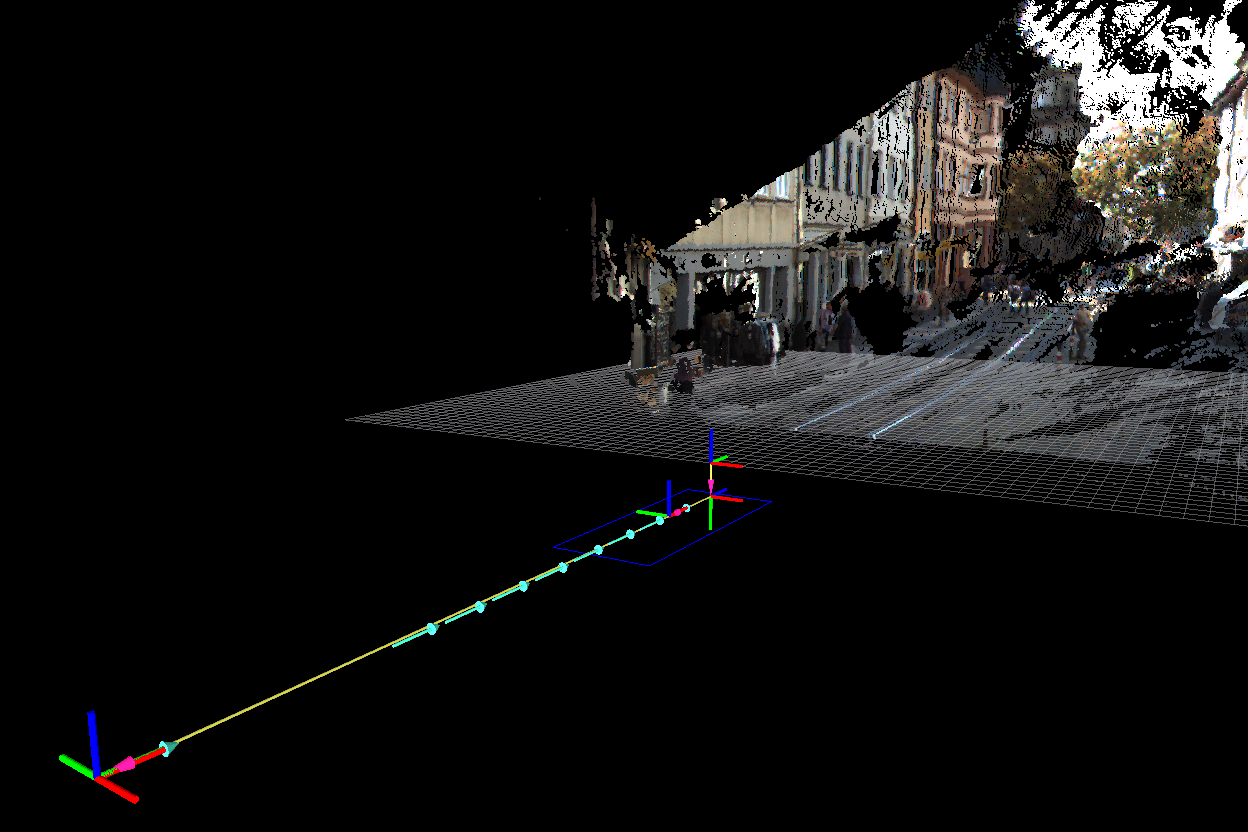
\includegraphics{tfs}
  \caption{Transformations tree used in our application. \todo{Añadir esquema con los frames arriba a la izquierda de la imagen} }\label{fig:cp05_tfs}
\end{figure}

\subsection{Voxelization}\label{ch:chapter05_01_03}

This is the first stage of the process of the process in charge of the object reconstruction. As said, we have implemented our application in four different processes in order to make it more modular. Three of them have been already described in the previous sections \ref{ch:chapter05_01_01}, \ref{ch:chapter05_01_01_01} and \ref{ch:chapter05_01_02}. This is the fourth.

As input, this process receives the odometry information obtained from the process described in \ref{ch:chapter05_01_02}, and the point cloud $\mathcal{P}$ obtained in section \ref{ch:chapter05_01_01_01}. This point cloud is processed, assigning each point $p_i = (p_x, p_y, p_z), i=1..N_p$ to the corresponding voxel $g_j=(g_w, g_l, g_h), j=1..N_g$, using the expression

\begin{equation}\label{eq:cp05_point_to_voxel}
\begin{cases}
g_w = (p_x - I_{min}(X)) / DX\\
g_l = (p_y - I_{min}(Y)) / DY\\
g_h = (p_z - I_{min}(Z)) / DZ
\end{cases}
\end{equation}

$N_p$ is the number of points in $\mathcal{P}$, $N_g = W * L * H$ is the total number of voxels in the grid $\mathcal{G}$ and $w$, $l$ and $h$ are the integer coordinates inside the grid at $X$, $Y$ and $Z$ dimensions. The grid is represented in the way that the centroid of the voxel $g_j=(0,0,0)$ is located at position $(I_{min}(X) - (DX/2), I_{min}(Y) - (DY/2), I_{min}(Z) - (DZ/2))$.

On each voxel, we store information related to:
\begin{itemize}
 \item The 3D associated points, assigned with the expression at equation \ref{eq:cp05_point_to_voxel}.
 \item The centroids $c=(c_x, c_y, c_z)$ of each voxel.
 \item Uncertainty of the stereo reconstruction values $\sigma_{x_{grid}}$, $\sigma_{y_{grid}}$ and $\sigma_{z_{grid}}$, which will be explained at section \ref{ch:chapter05_01_03_01}
 \item Weights $\omega_{occupied}$ and $\omega_{free}$, described also in the same section.
 \item Density of 3D points $N_p$.
 \item Main orientation and speed vectors $v=(v_x, v_y, v_z)$ and their associated yaw $\psi$, pitch $\theta$ and magnitude $\|v\|$.
 \item Stored particles $q_i = (x, y, z, v_x, v_y, v_z) \in \mathcal{Q}$, with their associated position $x$, $y$, $z$ and velocities $v_x$, $v_y$ and $v_z$.
 \item Obstacle identifier $o_i \in \mathcal{O}$, referencing the obstacle it belongs to. The process in which this identifier is assigned is described in section \todoref{XXX}.
\end{itemize}

\subsubsection{Conditional Probabilities Calculation}\label{ch:chapter05_01_03_01}

Both posterior and conditional probabilities of the received measurement are obtained a method similar to that described in \cite{isard1998condensation}, for a three-dimensional case, as that we have. Probabilities are directly related to the existence of not of 3D points in each one of the voxels. These probabilities will help us, in the next stages, to weight the particles.

For each voxel, we need to know the conditional probability of the associated measurements, under the occupied or free asumption. For that, we have to take into account the specificities of each sensor. In our case, we have based our tests on a stereo camera. In this kind of sensors, uncertainties grow while depth is bigger. So, we want to compute this uncertainty for the centroid $c=(c_x, c_y, c_z)$ associated to each voxel. Then, the uncertainty of the distance reconstruction is given by:

\begin{equation}\label{eq:cp05_uncertainty_distance_reconstruction}
\sigma_{c_y}={{{c_y}^2 \cdot \sigma_d} \over {b \cdot f}}
\end{equation}

Here, $\sigma_d$ is the error in disparity computation; $b$ is the baseline of the stereo system; and $f$ is the focal distance (in pixels).

Based on equation \ref{eq:cp05_uncertainty_distance_reconstruction}, we can derive the lateral and height positioning error $\sigma_w$ and $\sigma_h$:

\begin{equation}\label{eq:cp05_uncertainty_lateral_and_height_reconstruction}
\begin{align}
\sigma_{c_x}={{{c_x} \cdot \sigma_l} \over {c_y}} \\
\sigma_{c_z}={{{c_z} \cdot \sigma_l} \over {c_y}}
\end{align}
\end{equation}
These errors must be mapped into voxel errors. This is just done by dividing them with the voxel size on each dimension.

\begin{equation}\label{eq:cp05_uncertainty_voxel_errors}
\begin{align}
\sigma_w={{\sigma_{c_x}} \over {DX}} \\
\sigma_l={{\sigma_{c_y}} \over {DY}} \\
\sigma_h={{\sigma_{c_z}} \over {DZ}}
\end{align}
\end{equation}

Based on these errors, the idea is to find an approximation for the conditional probabilities of the measurement voxels under the occupied/free assumption. For that, we count the occupied neighbor voxels in the grid. The distance for which we consider a voxel as neighbor comes from the values of $\sigma_w$, $\sigma_l$ and $\sigma_h$. The total number of occupied neighbors is divided by the total number of voxels explored, obtaining the final value of the conditional probability.

\begin{equation}\label{eq:cp05_conditional_prob}
p(m(w,l,h)|occupied) = {
{\sum \limits_{w'=w-\sigma_w}^{w+\sigma_w} \sum \limits_{l'=l-\sigma_l}^{l+\sigma_l} \sum \limits_{h'=h-\sigma_h}^{h+\sigma_h} O(w',l',h')} 
\over 
{(2 \cdot \sigma_w + 1) \cdot (2 \cdot \sigma_l + 1) \cdot (2 \cdot \sigma_h + 1)}}
\end{equation}

, where

\begin{equation}\label{eq:cp05_occupied}
\begin{align*}
 O(w', l', h') &=
  \begin{cases}
   1        & \text{if } %
   %
   {\exists p(x, y, z) \in \mathcal{P} ~|~ p \text{ belongs to } \mathcal{G}(w', l', h')}%
   \\
   0        & \text{otherwise}
  \end{cases}
\end{align*}
\end{equation}

The conditional probability of the measurement given the “free” assumption is

\begin{equation}\label{eq:cp05_conditional_prob}
p(m(w,l,h)|occupied) = 1 - p(m(w,l,h)|free)
\end{equation}

In figure \ref{fig:cp05_voxelization} the obtained voxels are represented. The occupation probability is represented through the alpha channel of each of them, so the opacity is directly related to this probability, being the most transparent ones those with a low value.

\begin{figure}[th]
  \centering
  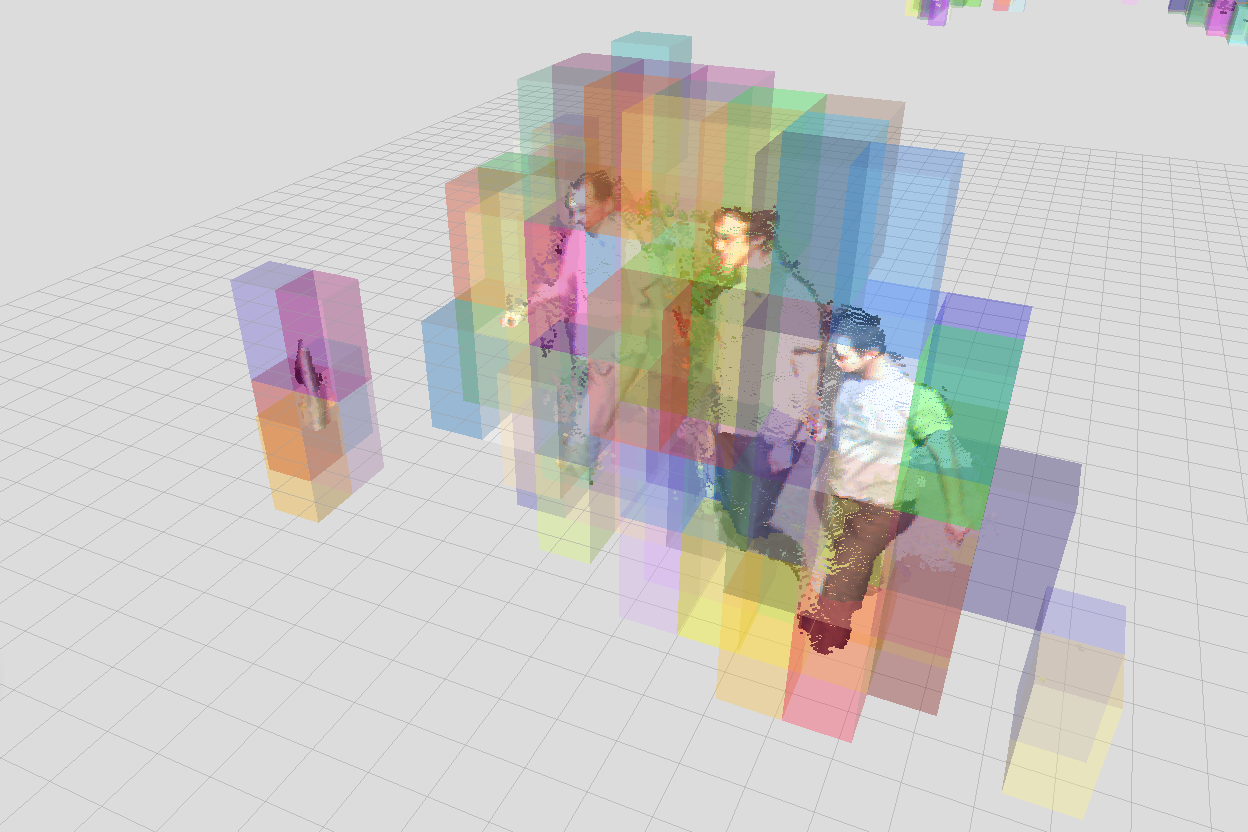
\includegraphics{voxelization}
  \caption{Voxelization of a given point cloud. Those voxels with a bigger occupation probability are more opaque.\todo{Poner opacidad en función de la probabilidad} }\label{fig:cp05_voxelization}
\end{figure}

\subsection{Voxel pose and speed computation}\label{ch:chapter05_01_04}

The pipeline of this step is represented in figure \ref{fig:cp05_voxel_pose_speed_computation}. One of the advantages of using a grid of voxels is that most of the computation is performed for each of them separately, making it suitable for a parallel implementation. 

An explanation of the subtasks of this step is given next:

\begin{figure}[th]
  \centering
  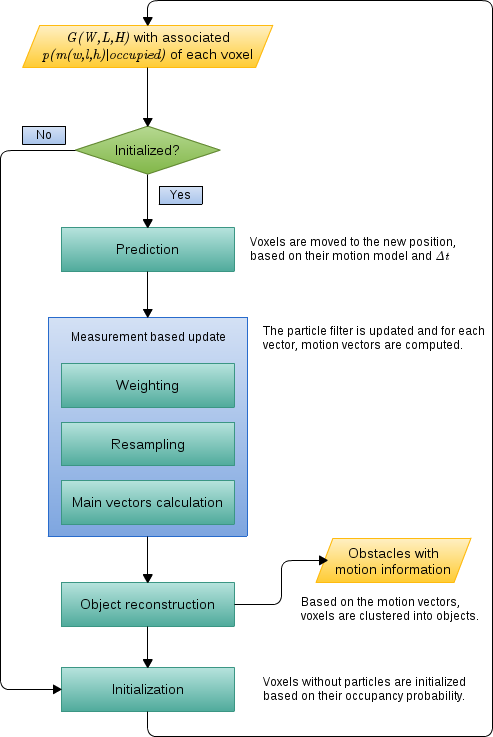
\includegraphics{voxelPoseAndSpeedComputation}
  \caption{Pipeline of the voxel pose and speed computation stage.}\label{fig:cp05_voxel_pose_speed_computation}
\end{figure}

\subsubsection{Prediction}\label{ch:chapter05_01_04_01}

In this step, we compute the present particle distribution taking into account each particle motion model and the time that has passed between frames. With this new distribution, data will be ready for the next task. In the method developed by \cite{danescu2012particle}, they updated the particle set in a step quite similar to this one. However, in their work, prediction equations used odometric information in order to compensate the ego-motion. In our approach, we do not perform this compensation. This doesn't means that we do not care about our the bias introduced by the vehicle movement, but this movement will be compensated at the end of the process, once we have the orientation and speed of each obstacle. This come with some avantages:
\begin{itemize}
 \item We do not need to translate and rotate the whole grid between iterations, as it is moving together with the left camera based frame.
 \item We just need to apply the motion equations in order to update the particles set.
\end{itemize}

These advantages allows saving a lot of resources. This is the most computationally expensive of the tasks in the method, which is highly dependent on the parameter $N_g$, that controls the number of particles. If we speed up this step, the system will be able to deal with a larger number of particles, improving the results.

Each of the particles $q_i = (x, y, z, v_x, v_y, v_z) \in \mathcal{Q}$ is updated as follows. First, we need a motion model that allows to transform the particles based on the increment of time $\Delta t$ and the parameters of position and speed of the particle. For this purpose, we introduce the state transition matrix $S$:

\begin{equation}\label{eq:cp05_state_transition_matrix}
S =
\left( \begin{array}{cc}
I_{3\times3} & \Delta t \cdot I_{3\times3} \\
0_{3x3} & I_{3\times3} \end{array} \right)
\end{equation}

We also introduce the matrix $\Delta$, which models the stochastic diffusion caused by the uncertainties in the motion model.

\begin{equation}\label{eq:cp05_state_motion_model_uncertainties}
\Delta =
\left( \begin{array}{cccccc}
\delta x & \delta y & \delta z & \delta v_x & \delta v_y & \delta v_z
\end{array} \right)^T
\end{equation}

Here, $\delta x$, $\delta y$, $\delta z$, $\delta v_x$, $\delta v_y$ and $\delta z$, are randomly drawn from a Gaussian distribution of zero mean and a covariance matrix Q equivalent to the state transition covariance matrix of a Kalman filter.

So, the new position of each particle is given by the expression

\begin{equation}\label{eq:cp05_particle_update}
q_{t + 1} = S \cdot q_{t} + \Delta
\end{equation}

\subsubsection{Weighting and resampling}\label{ch:chapter05_01_04_02}

This step is quite similar to the stage with the same name in the work of \cite{danescu2012particle}, with some minor differences, most of them related to the addition of a new dimension. For optimization reasons, in this stage we also perform the calculation of the main orientation and speed vectors associated to each voxel.

As said before, particles are the base of our system. They are used both as hypotheses and as the building blocks of the different obstacles. From these particles, we are going to calculate the main vectors of each voxel, which will be used in later steps for the reconstruction and segmentation of the final obstacles.

But in this step we are more interested in their role as hypotheses. A particle in a voxel is a hypothesis saying that it is occupied, and that it has the speed equal to the speed of the particle. The more particles in a voxel, the more chances to be occupied. If there are not many particles in the voxel, the hypothesis of the voxel being free is supported. The particles are multiplied or deleted depending on how well the occupied or the free hypotheses of each voxel are supported by the measured data.

This step is composed by two steps: Weighting and Resampling. As said, we also include the main vectors calculation in this section, but it could be easily a separate step which is included here just for optimization reasons.

\paragraph{Main vectors calculation}\label{ch:chapter05_01_04_02_01}

Once the survival particles which fall inside an occupied voxel have been computed, main vectors are obtained. The way in which we do that is through an spherical histogram. The idea, depicted in figure \ref{fig:cp05_spherical_hist}, works at follows:
\begin{itemize}
 \item The possible values of yaw $\psi$ that the voxel can take ($[0\dots2\pi]$) is divided in intervals of size $\Delta\psi$; we do the same for the pitch $\theta$, with intervals of size $\Delta\theta$. In our tests, both $\Delta\psi$ and $\Delta\theta$ are set to $5^{\circ}$.
 \item For each particle, we obtain the corresponding value of $\psi$ and $\theta$, and the corresponding bin is increased in one unit. Each bin stores, also, the average of the speeds related to each particle.
 \item The speed and orientation will be given by the bin with the biggest number of related particles.
 \end{itemize}
 
 After this process, each voxel will know their estimated speed and direction. These must be obtained using just the surviving particles after the prediction process. As weighting and resampling is an stochastic process, results could be biased by wrongly duplicated or eliminated particles. In figure \ref{XXX-segmentation} we can view the main vectors obtained for the surviving voxels after the segmentation process.

\begin{figure}[th]
  \centering
  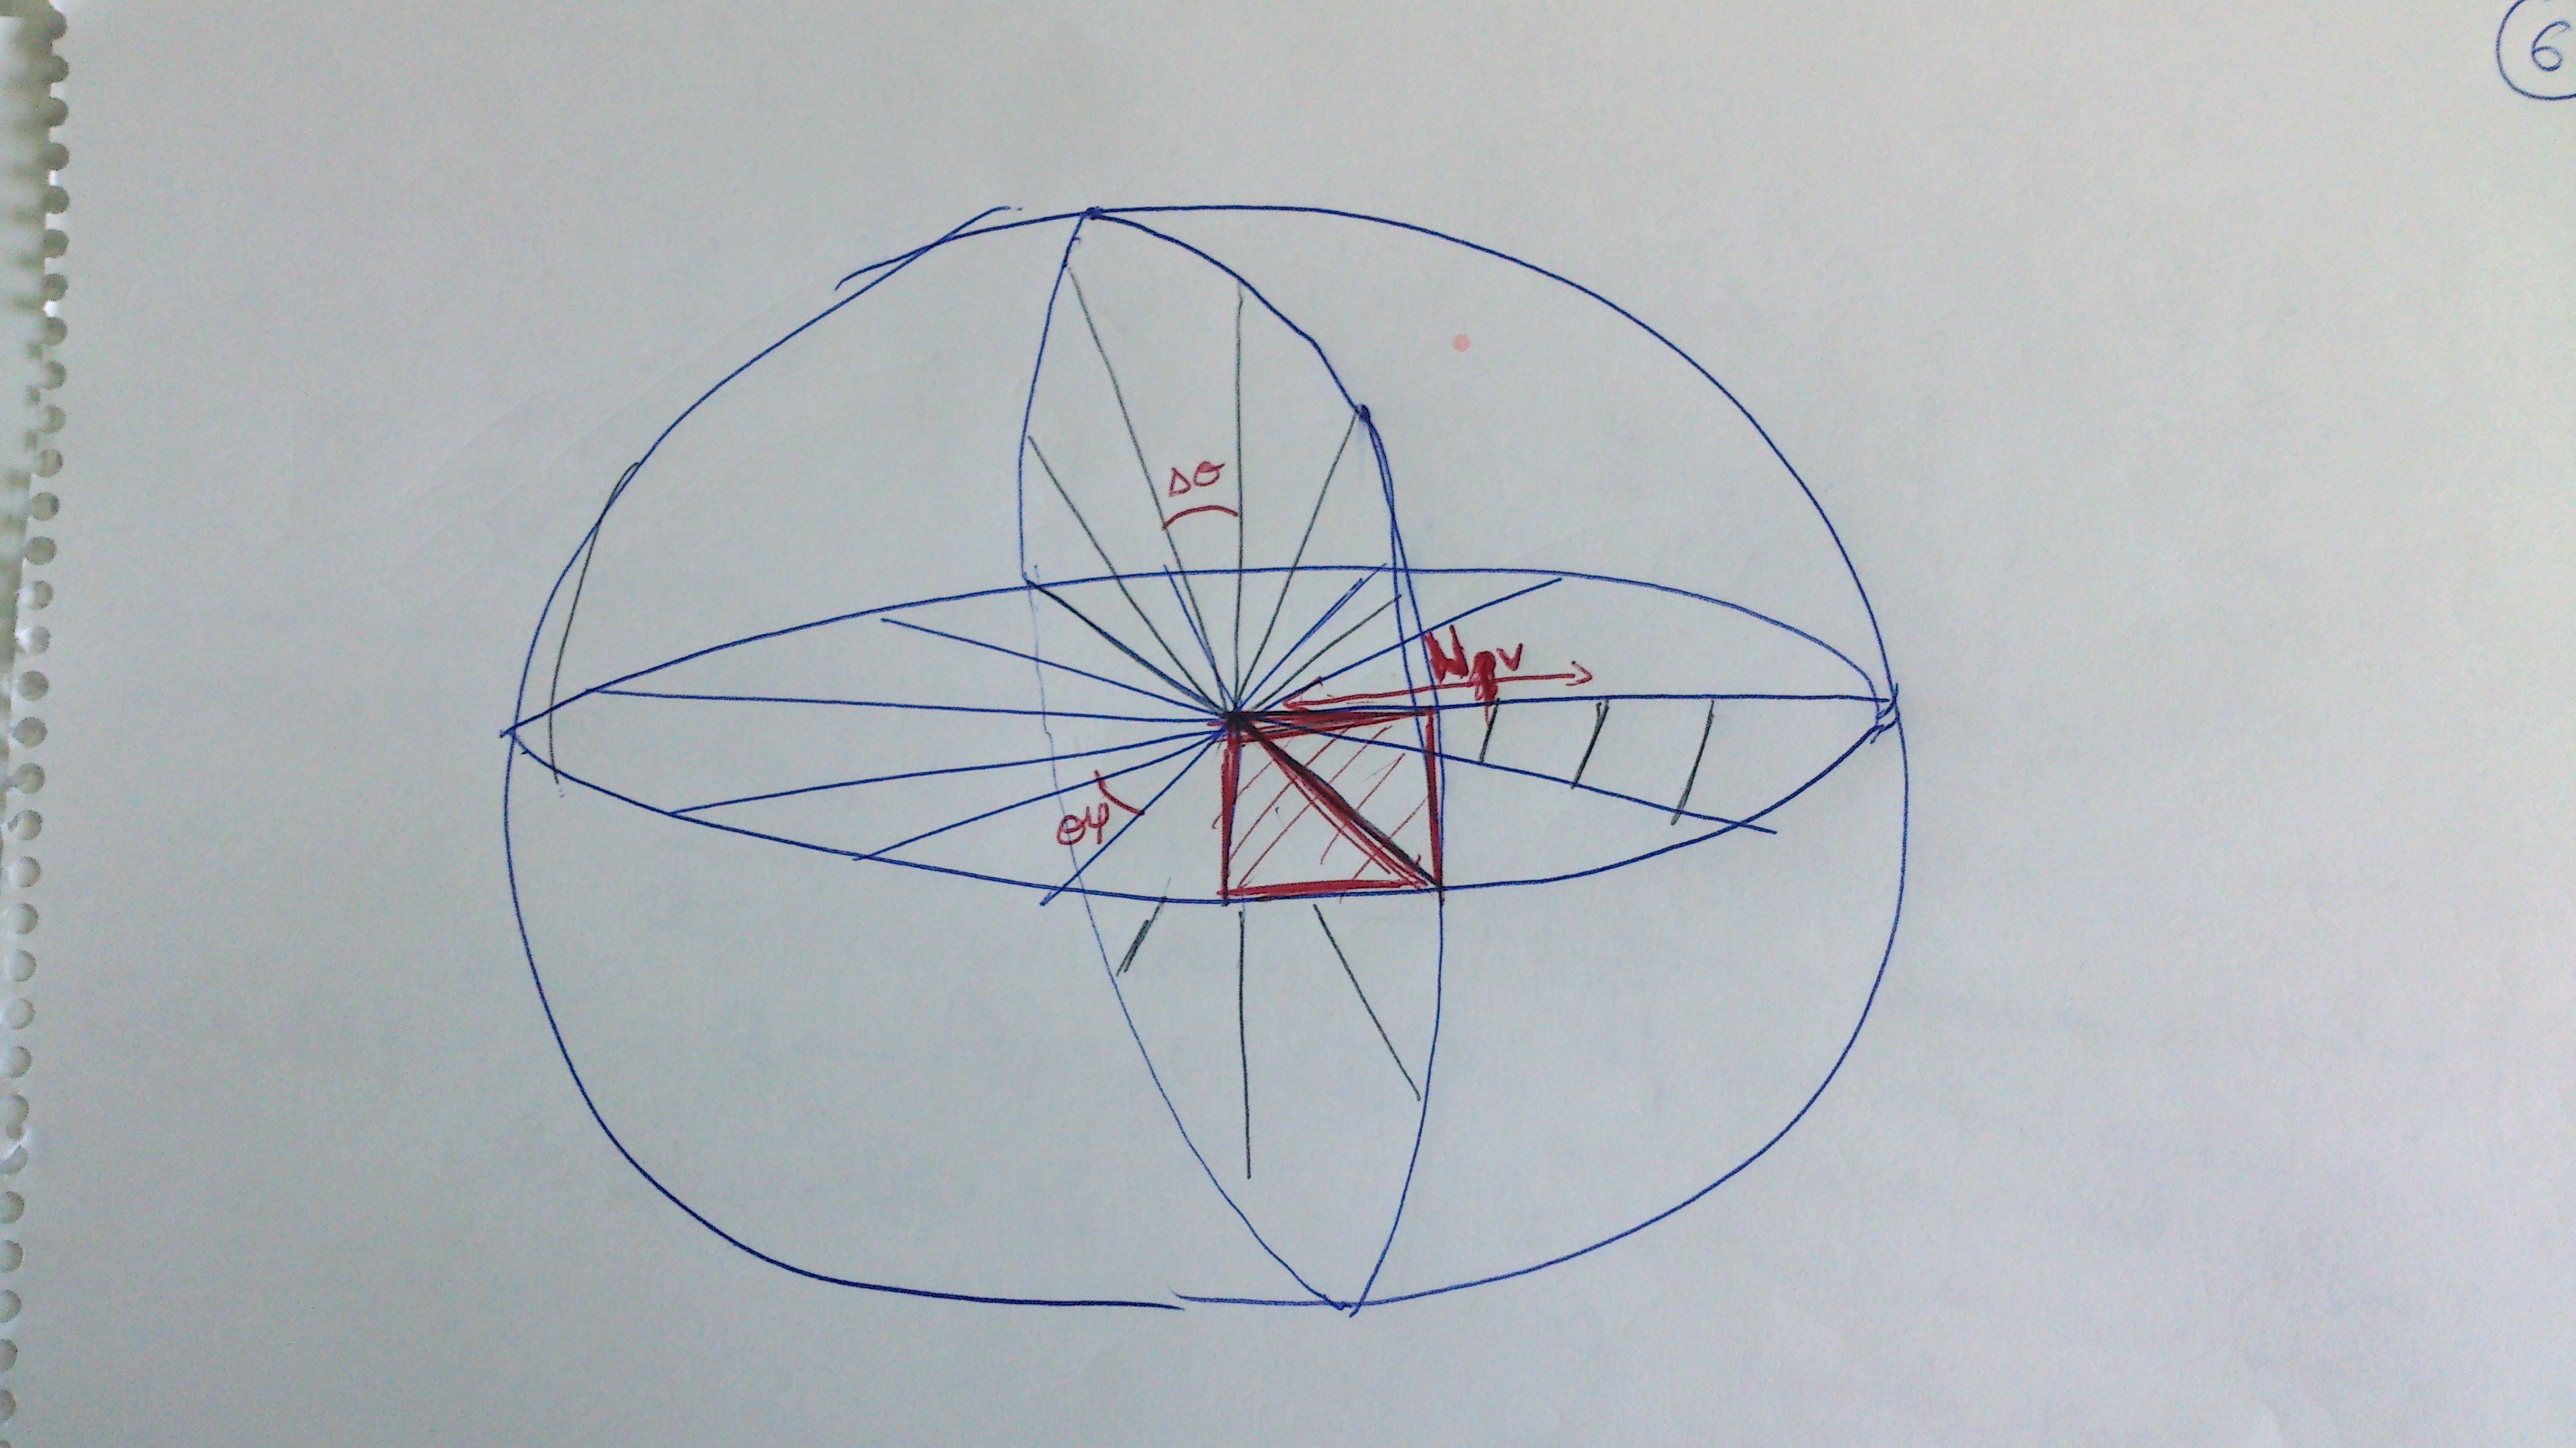
\includegraphics{sphericalHist}
  \caption{Diagram representing an spherical histogram.}\label{fig:cp05_spherical_hist}
\end{figure}

\paragraph{Weighting}\label{ch:chapter05_01_04_02_02}

The number of particles $N_g$ is assumed to be constant, assuming that the real particles inside a voxel have the occupancy value \emph{true}, while that the absence of real particles is considered as the presence of virtual particles with an occupancy value equal to \emph{false}. Based on this idea, as measurement data does not include speed information (we are using as input pure 3D point clouds), the weight of the particles depends only on the \emph{occupied} hypothesis.

So, for each voxel, we are interested on getting the total posterior probability of being occupied or free. In order to obtain these probabilities, we will need the measurement conditional probabilities (weights) of each voxel and the number of free/occupied hypotheses. The total posterior probabilities are given by:

\begin{equation}\label{eq:cp05_total_posterior_probabilities}
\begin{array}{l}
P_{og}={{\omega_{occupied} \cdot N_{og}} \over {\omega_{occupied} \cdot N_{og} + \omega_{free} \cdot N_{fg}}} \\
P_{fg}={{\omega_{free} \cdot N_{fg}} \over {\omega_{occupied} \cdot N_{og} + \omega_{free} \cdot N_{fg}}}
\end{array}
\end{equation}

In these equations, the values of the weights $\omega_{occupied}$ and $\omega_{free}$ are already calculated during the process described at section \ref{ch:chapter05_01_03_01}, so 

\begin{equation}\label{eq:cp05_occupancy_weights}
\begin{array}{l}
\omega_{occupied} = p(m(w,l,h)|occupied) \\
\omega_{free} = p(m(w,l,h)|free)
\end{array}
\end{equation}

; about $N_{og}$ and $N_{fg}$, they are the number of particles having the \emph{occupied} hypothesis (real number of particles in the voxel), and those having the \emph{free} hypothesis, respectively. As said before, we consider the absence of particles as the presence of a set of virtual particles with the hypothesis \emph{free}:

\begin{equation}\label{eq:cp05_number_of_particles}
\begin{array}{l}
N_{og} = | \{ p_i \in \mathcal{P} | p_i \text{ belongs to voxel } g \} | \\
N_{fg} = N_g - N_{og}
\end{array}
\end{equation}

\paragraph{Resampling}\label{ch:chapter05_01_04_02_03}

After the weighting step is done, we can start with the resampling step. After this, the population of particles will be properly updated, so we can use them for the reconstruction of the obstacles. As we do not take into account the free voxels, just real particles (those with the \emph{occupied} hypothesis) will be considered. For each of these particles, we will decide if they are destroyed or multiplied. After the process of resampling has been completed, each voxel will have the proper number of particles.

In the algorithm \ref{alg:cp05_weighting_resampling}, we describe the resampling process. For the sake of clarity, the point in which weighting and main vectors are computed is indicated.

\begin{algorithm}
\caption{Weighting and Resampling}
\label{alg:cp05_weighting_resampling}
\begin{algorithmic}
\State {\comment{A la persona que me esté revisando esto: échale un ojo al algoritmo correspondiente en \cite{danescu2012particle} (pagina 11). No se si es plagio o adaptacion al caso concreto de los voxels y, en parte, a como llevé el cambio de celda a voxel. En general es el mismo algoritmo, pero uní los dos fors por un tema de optimización: no recorro todas las partículas correspondientes buscando el voxel asociado. En vez de eso, recorro para cada voxel (para el cual ya calculé $f_g$) y hago el resampling sólo en las partículas asociadas. A efectos prácticos es lo mismo, sólo que más eficiente :) }}
\Function{MeasurementBasedUpdate}{$\mathcal{G}$} 
  \For {\textbf{each} voxel $g \in \mathcal{G}$}
    \State \textbf{Main vectors computation}
      \State \indent {$g$.computeMainVectors()}
    \State
    \State \textbf{Weighting}
      \State \indent Compute $N_{og}$ and $P_{og}$
      \State
    \State \textbf{Resampling}
      \State \indent Compute resampled number of particles $N_{rg}$
      \State \indent $N_{rg} \gets P_{og} \cdot N_g$
      \State \indent $f_g \gets {{N_{rg}} \over {N_{og}}}$
    \For {\textbf{each} particle $p$ belonging to $g$}
      \State \Comment { The number of particles will be increased.}
      \If { $f_g > 1$ } 
	\State {$F_n \gets \lfloor f_g\rfloor$} \Comment {Integer part}
	\State {$F_f \gets f_g - \lfloor f_g\rfloor$} \Comment {Fractional part}
	\For {$k = 1$ to $F_n - 1$}
	  \State {$g$.makeCopy($p$)}
	\EndFor
	\State $r \gets \text{random value in the range [0 \ldots 1]}$
	\If {$r < F_f$}
	  \State {$g$.makeCopy($p$)}
	\EndIf
      \State \Comment {$f_g < 1$, the number of particles will be decreased.}
      \Else 
	\State $r \gets \text{random value in the range [0 \ldots 1]}$
	\If {$r > F_g$}
	  \State {$g$.remove($p$)}
	\EndIf
      \EndIf
    \EndFor
  \EndFor
\EndFunction
\end{algorithmic}
\end{algorithm}

The algorithm is almost the same as proposed in \cite{danescu2012particle}. The main difference is that, due to optimization reasons we do not split the whole process into two different loops. To do that, instead of having the set of particles separated from the voxels, each voxel knows exactly where its particles are. In the original algorithm, it is necessary to compute and store the value of $f_g$ for absolutely all the voxels in $\mathcal{G}$. After that, the program iterates over all the particles in $\mathcal{P}$. For each of these particles $p$, we need to know the related voxel and look for the computed value $f_g$. In our approach, we assign each particle to its voxel directly at the \emph{initialization} and \emph{prediction} steps, so we can perform all the weighting and resampling step at once, saving a little bit more computational time again.

The resampling process depends on the value of the ratio between the actual number of particles and the number of resampled particles ($f_g$). Based on this value, we know if the particles will be duplicated ($f_g > 1$) or removed ($f_g < 1$). In figure \ref{fig:cp05_weight_and_resample}, an example where the surviving particles after this step are shown. In this case, pedestrians are moving in the negative direction of $X$ and $Y$ axis, so the most of surviving particles have this trend. These will be used in the next step for the calculation of the main vectors representing the movement of each voxel separately.

\begin{figure}[th]
  \centering
  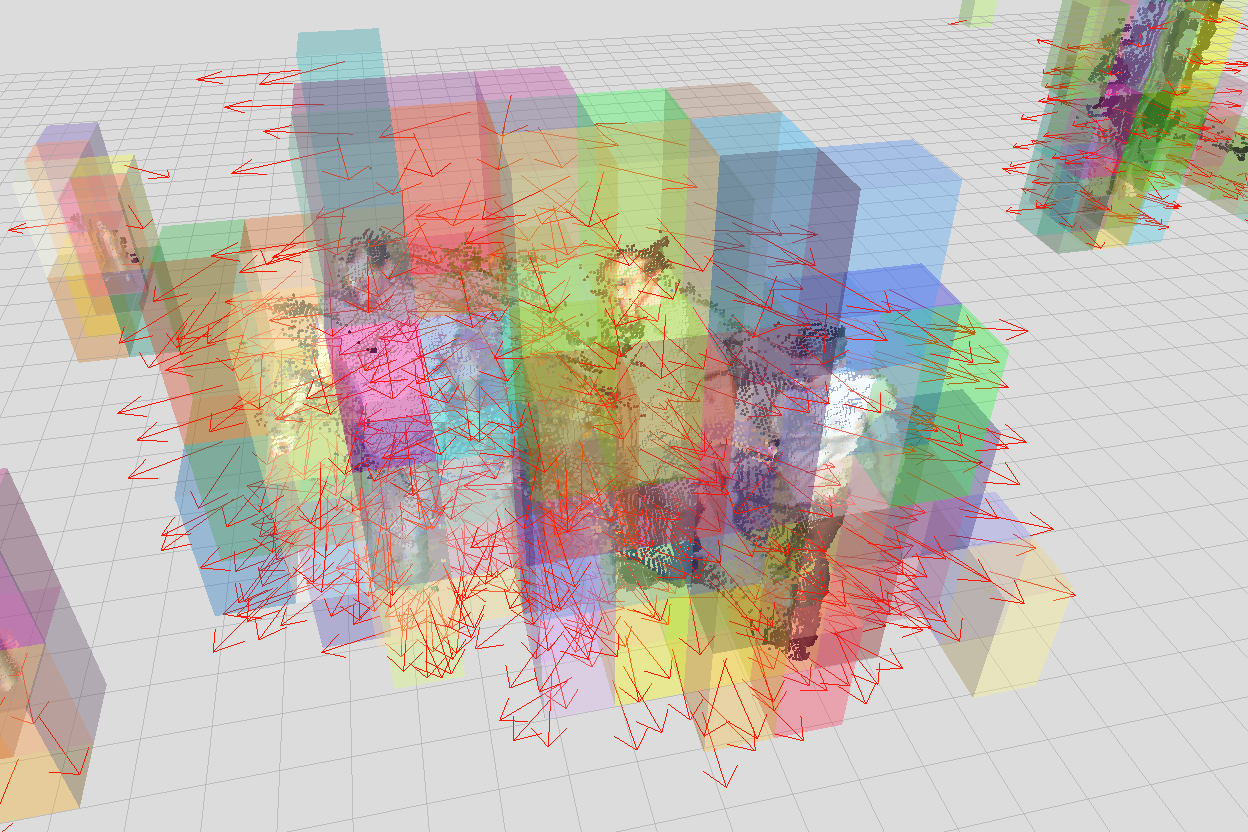
\includegraphics{weightAndResample}
  \caption{Pipeline of the voxel pose and speed computation stage.}\label{fig:cp05_weight_and_resample}
\end{figure}

After this process is finished, we can proceed to the initialization stage.

\subsubsection{Initialization}\label{ch:chapter05_01_04_03}

In this stage, those voxels without particles initialize a new set of them with a number proportional to the occupancy probability. This situation can be reached for two reasons:
\begin{itemize}
 \item This is the first iteration, so none of the voxels has been initialized already.
 \item After the weighting and resampling process, none of the particles survived.
\end{itemize}

This stage is the first step we perform in the execution on the method, and the last at each iteration. It is in charge of ensuring that the number of particles never become zero. Here, we just check each of the voxels $g \in \mathcal{G}$. If there are not particles in the voxel ($N_p = 0$), or the occupancy probability is bigger than the occupancy threshold $\tau_{o}$ ($\omega_{occupied} > \tau_{o}$), a number of particles equal to $N_p$ is initialized in the voxel.

Given the voxel $g \in \mathcal{G}$, each particle is initialized with the position $(x, y, z) = (g.c_x, g.c_y, g.c_z)$, and a random speed $(v_x, v_y, v_z)$ in the range $[0\dots v_{max}(n)]$, being $v_{max}(n)$ an user defined parameter that determines the maximal speed at each dimension $n \in \{ X, Y, Z\}$ that is expected by each voxel. 

In this implementation, we allow vertical movements controlled by the parameter $v_{max}(Z)$. However, in certain situations like planar grounds this movement is not relevant, so it is better to assign it to $0$, so the particles can restrict their movement to the $XY$ plane.

\subsection{Object reconstruction}\label{ch:chapter05_01_05}

Based on the main vectors obtained for each voxel, we can assume that all the adjacent voxels with a similar direction and speed belong to the same obstacle, or at least to the same group of obstacles (for example, we could find a situation in which a group of people are all of them walking together. We are not concerned about this case because if they are considered as a single obstacle is because they are adjacent and there is no traversable space between them. As they walk in the same direction, in practice we can think on them as a single obstacle).

In this sense, we have developed a method inspired in the color-based clustering described by \cite{broggi2013}. However, in our case, the similarity function is not based on color information because of the reasons explained before, so this similarity function is split into three different similarity functions:

\begin{equation}\label{eq:cp05_similarity_functions}
\begin{array}{l}
f_1(o,g)=\| |\vec{v}|_o - |\vec{v}|_g \|\\
f_2(o,g)=\| \phi_o - \phi_g \|\\
f_3(o,g)=\| \theta_o - \theta_g \|
\end{array}
\end{equation}

, where $|\vec{v}|_o$ and $|\vec{v}|_g$ are the modulus of the speeds obtained for an obstacle $o \in \mathcal{O}$ and for a voxel $g \in \mathcal{G}$, respectively. The same applies for the yaw $\phi_o$ and $\phi_g$, and the pitch $\theta_o$ and $\theta_g$ measurements.

The use of these similarity functions has several advantages. The most direct is that the input cloud of our algorithm can be generated by a sensor different from a stereo pair. We could even combine them, as it has been said before. The employed flood-fill based clustering algorithm is described in the algorithm \ref{alg:cp05_clustering}.

\begin{algorithm}
\caption{Clustering algorithm}
\label{alg:cp05_clustering}
\begin{algorithmic}
\Function{Clustering}{$\mathcal{G}$} 
\State {$\mathcal{G'} \gets \mathcal{G}$} \Comment {$\mathcal{G'}$ is the set of not-checked voxels. }
\For {\textbf{each} voxel $g \in \mathcal{G'}$}
  \State {$\mathcal{G'} \gets \mathcal{G'} - g$}
  \State {$o \gets \text{ new object containing }g$}
  \State {$\text{insert } g \text{ in } queue$}
  \While {$queue \ne \emptyset$}
    \State {$g' \gets \text{extract first element from the } queue$}
    \For {\textbf{each} $\{ g'' | g'' \in o\} \in N(g')$}
      \If {$ f_1(o,g) < \tau_{v} \textbf{ and } f_2(o,g) < \tau_{\psi} \textbf{ and } f_3(o,g) < \tau_{\theta} $}
	\State {$\text{insert } g'' \text{ in } o$}
	\State {$\text{insert } g'' \text{ in } queue$}
      \EndIf
    \EndFor
  \EndWhile
  \If {$|o| >= \tau_{min\_voxels\_per\_obstacle} \textbf{ and }$\\ 
  \pushcode\pushcode$~~~~o.sz(Z) >= \tau_{min\_obstacle\_height} \textbf{ and }$\\
  \pushcode\pushcode$~~~~o.min(Z) == I_{min}(Z)$}
      \State {$o \text{.updateVectors()}$}
      \State {$\text{insert } o \text{ in } \mathcal{O}$}
  \EndIf
\EndFor
\EndFunction
\end{algorithmic}
\end{algorithm}

The neighborhood of a voxel $g$ represented by the function $N(g)$, as in \cite{broggi2013}, is performed using the Chebyshev distance. When a new voxel $g''$ is added to an obstacle $o$, the voxel identifier is updated. From the obstacle point of view, we just add the voxel to a list associated to each obstacle. Once an obstacle is about to be added to the final set of obstacles, this list will be used for updating the information related to the obstacle centroid, speed and limits on each dimension (See section \ref{ch:chapter05_01_05_01}).

Before adding an obstacle to the final list of obstacles $\mathcal{O}$, we perform a filtering stage which, for optimization reasons, has been integrated in the segmentation process. This filtering procedure is based in a set of assumptions, related to the expected size of the obstacles and their position regarding to the ground. An obstacle is accepted in the final list if:

\begin{itemize}
 \item It is big enough. That is, if the number of voxels (which is directly proportional to its volume) is over the user-defined parameter $\tau_{min\_voxels\_per\_obstacle}$.
 \item It is tall enough. The minimal height is controlled by the parameter $\tau_{min\_obstacle\_height}$
 \item The obstacle is on the ground. This helps to remove flying obstacles like traffic lights or the top of some trees.
\end{itemize}

\subsubsection{Obstacle vectors computation}\label{ch:chapter05_01_05_01}

Once we have the list of voxels that compose each obstacle, we can use it for the calculation of their speed direction and magnitude. We want also to compensate the motion of our vehicle in order to know their real speed. Let $ego_{vx}$, $ego_{vy}$ and $ego_{vz}$ be the vectors that represent the motion of the vehicle regarding to the left camera coordinates frame. Also, $o_{vx}$, $o_{vy}$ and $o_{vz}$ will be the motion vectors of each obstacle and $g_{vx}$, $g_{vy}$ and $g_{vz}$ those for each of the voxels in the list for that obstacle. Then, the final speed for each obstacle will be obtained by applying:

\begin{equation}\label{eq:cp05_obstacle_vectors_computation}
\begin{cases}
o_{vx} = {{\sum\limits_{g \in \mathcal{G}_o} g_{vx}} \over {|\mathcal{G}_o|}} + ego_{vx}\\
o_{vy} = {{\sum\limits_{g \in \mathcal{G}_o} g_{vy}} \over {|\mathcal{G}_o|}} + ego_{vy}\\
o_{vz} = {{\sum\limits_{g \in \mathcal{G}_o} g_{vz}} \over {|\mathcal{G}_o|}} + ego_{vz}
\end{cases}
\end{equation}

Here, $\mathcal{G}_o$ is the list of voxels associated to the obstacle $o$. In figure \ref{fig:cp05_obstacle_vectors_computation}, we have shown a simulation of which will be the future movement of the obstacles if we consider the obstacle speed computed in this stage.

\begin{figure}[th]
  \centering
  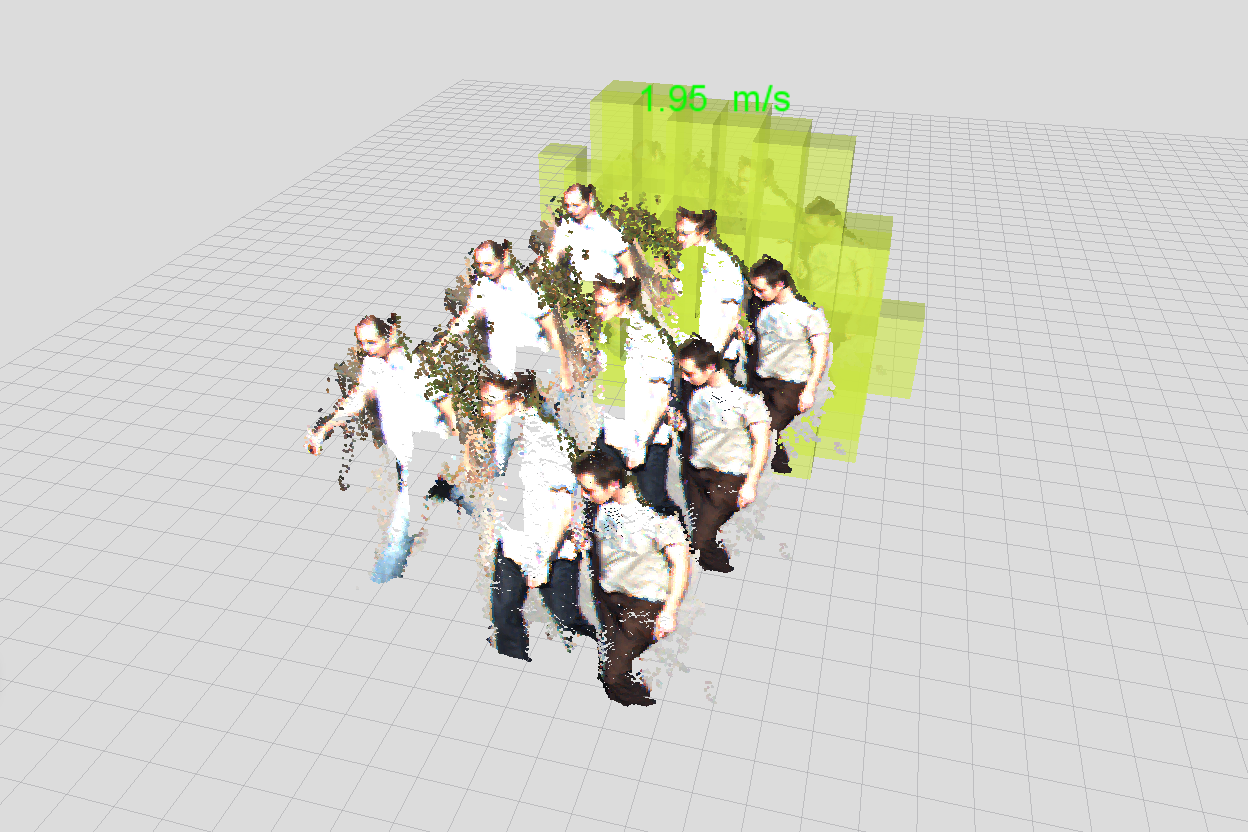
\includegraphics{fakePointCloud}
  \caption{Simulation of the obstacles future movement using the computed vectors.}\label{fig:cp05_obstacle_vectors_computation}
\end{figure}

\subsection{Planning and obstacle avoidance}\label{ch:chapter05_01_06}

\todo{Si me da tiempo, intentar meter el dataset de Daimler y hacer unos test de detection rate un poco mejores, incluyendo velocidades.}
The speed vectors of each obstacle, together with their position and the 3D point cloud stored by the associated voxels will be used by the planner of the vehicle in order to perform an efficient and safe planning. This task, which is the final objective of this thesis, will be described in section \todoref{XXX}. A figure of the output of this method being used for planning tasks is shown at figure \todoref{XXX}, in the same section. Also, a video of the pipeline of the whole method described here is available at \todoref{XXX}.

\section{Results}\label{ch:chapter05_02}

In this section, a few representative results of the behavior of our algorithm are shown. These results are divided in four sections. In the first one, we evaluate the best choice for the generation of the input point cloud, taking in consideration some of the results obtained in section \todoref{XXX-stereoeval} and some specific evaluations for the current application. The second section evaluates the quality of the ego-motion estimation. The last two sections are related to the detection quality and the performance shown by our method.

\section{Input point cloud}\label{ch:chapter05_02_01}

In this section, we describe the tests performed in order to choose the algorithm that we later used for the rest of evaluations shown in this chapter. If we look again to the charts in section \todoref{fig:cp05_tfs}, we notice that the response is similar for both algorithms in the chart at \todoref{XXX-LGT,density,alg}, where the density of all the algorithms is compared for the \ac{LGT} based evaluation. The same happens in the \todoref{XXX-alg,NCC}, despite we concluded that the reliability on this measure is still not clear. In chart \todoref{XXX-alg,NFC} the difference between both algorithms starts becoming bigger, with better results for the \emph{BT-SGM} approach if compared to the \emph{ELAS}. Anyway, results for this last method are not so bad, which is quite better if we attend to the average error computed using the \ac{LGT} (See chart at figure \todoref{XXX,LGT,avg}). This last measure is quite decisive, as too much noise can fake the results. If we look at figure \ref{fig:cp05_comparison_bt_sgm_vs_elas}, it is possible to see that the noise generated by \emph{BT-SGM} is much more than that by \emph{ELAS}. One of the reasons fo which this noise is not so strong is that the triangulation-based reconstruction of the disparity map used in \emph{ELAS} filters a lot of this noise. If we look at the street light, we can see that it is fully reconstructed in the right image (\emph{ELAS}), while the \emph{BT-SGM} is just able to do the reconstruction of the top of it. Of course, there is some depth imprecisions for the \emph{ELAS} example, but it is inside the range our algorithm is able to deal with. First, the variation is not bigger than the size of the base of our voxels, so the problem is minimized by this factor. Moreover, the use of the conditional probability of the measurement computed with the equation \ref{eq:cp05_conditional_prob} as the basis for the weight computation for each voxel also reduces the problems that could be associated by this kind of noise.

\begin{figure*}[th]
        \centering
        \begin{subfigure}[b]{0.475\textwidth}
                \centering
                \caption{BT-SGM}
                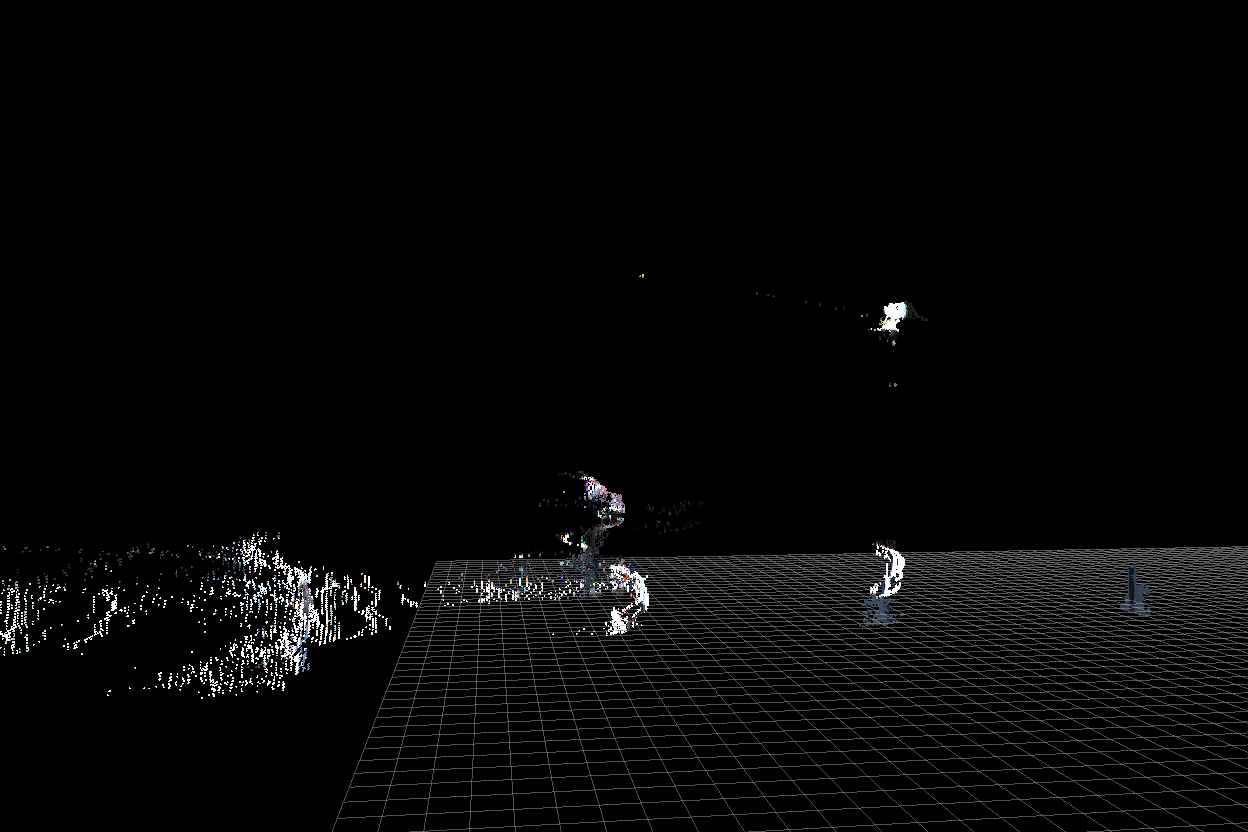
\includegraphics[width=\textwidth]{btsgm}\label{fig:cp05_bt_sgm}
        \end{subfigure}%        
        ~ 
        \begin{subfigure}[b]{0.475\textwidth}
                \centering
                \caption{ELAS}
                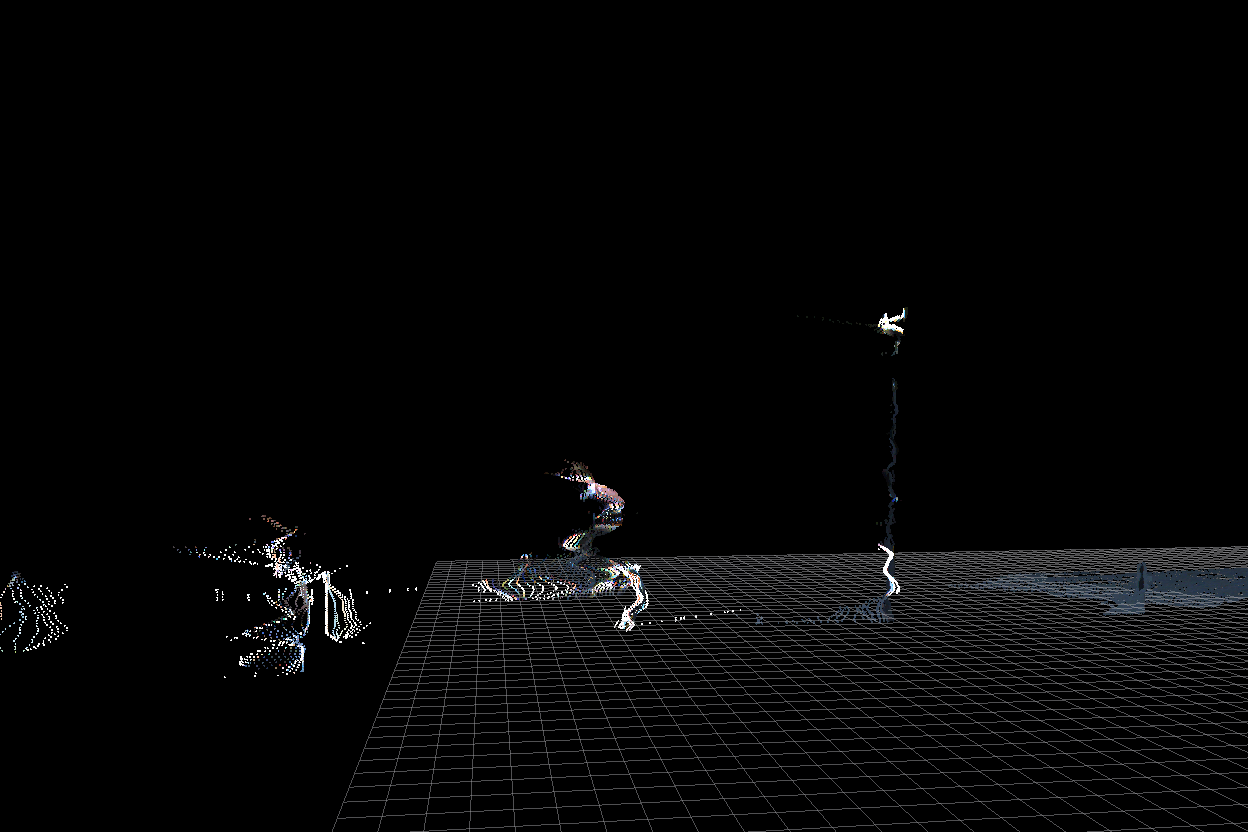
\includegraphics[width=\textwidth]{elas}\label{fig:cp05_elas}                
        \end{subfigure}%
        \caption{Comparison of a resulting point cloud obtained using both \emph{BT-SGM} and \emph{ELAS}.}\label{fig:cp05_comparison_bt_sgm_vs_elas}
\end{figure*}

If we look at figure \ref{fig:cp05_times_elas_btsgm}, we have represented the times obtained for each frame along a long sequence, where it is possible to appreciate that \emph{ELAS} is much faster than \emph{BT-SGM}. In this test, the average frequency obtained by the former is about $17\,Hz$, while the second is able to work at an average below $5\,Hz$ in the implementation used. For the application described, we require a fast algorithm in order to complete the whole pipeline in real time. Considering the fact that the differences in reconstruction quality are not so big between them (with some good results for \emph{ELAS}), and the big differences in time performance, we chose to use the \emph{ELAS} algorithm as the base for the point cloud reconstruction step.

 \begin{figure}[th]
  \centering
  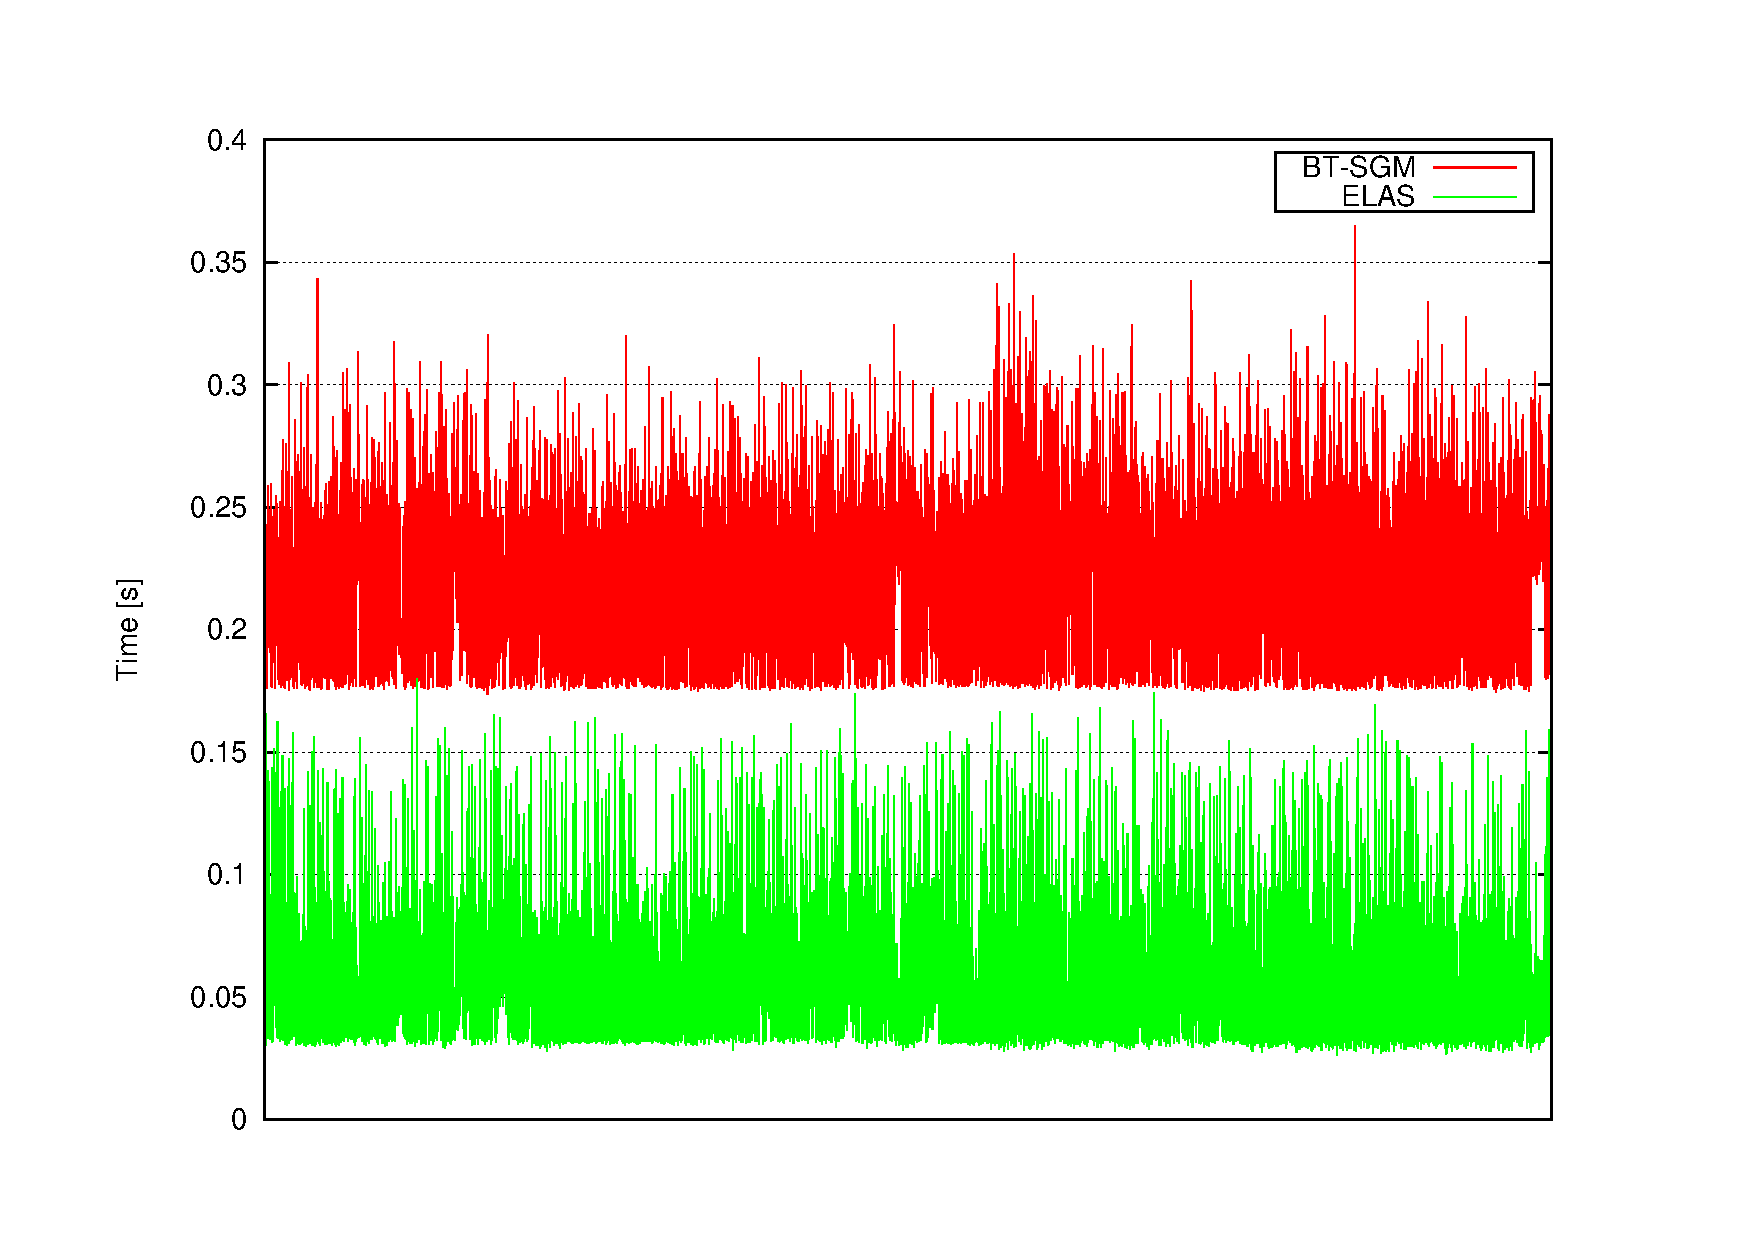
\includegraphics[trim=50 50 90 60, clip]{timesELAS_OPENCV}
  \caption{Comparison of the required time for each of the stereo reconstruction algorithms.}\label{fig:cp05_times_elas_btsgm}
\end{figure}

\section{Ego-motion}\label{ch:chapter05_02_02}

In this section, we want to know if using visual odometry or mechanical odometry could affect to the rest of the pipeline. To do that, we have chose one of the sequences in the Karlsruhe KITTI Dataset (\cite{geiger2013vision}), for which a sequence of stereo pair of images is available. For each of these images, the mechanical odometry information is available, as well as the time in which these images were captured.

With this information, we computed the yaw increment between frames, as well as an estimation of the speed on each frame (by computing the distance to the previous frame and dividing it by the time between frames). At the same time, we compute the visual odometry using the method of \cite{geiger2011stereoscan}, and the same process is performed using the output of the algorithm. Results are shown in figures \ref{fig:cp05_ego_yaw} and \ref{fig:cp05_ego_speed}.

If we look at the yaw comparison chart in figure \ref{fig:cp05_ego_yaw}, we observe that the difference between both methods is minimal, where the maximal difference of below 0.001 radians.

 \begin{figure}[th]
  \centering
  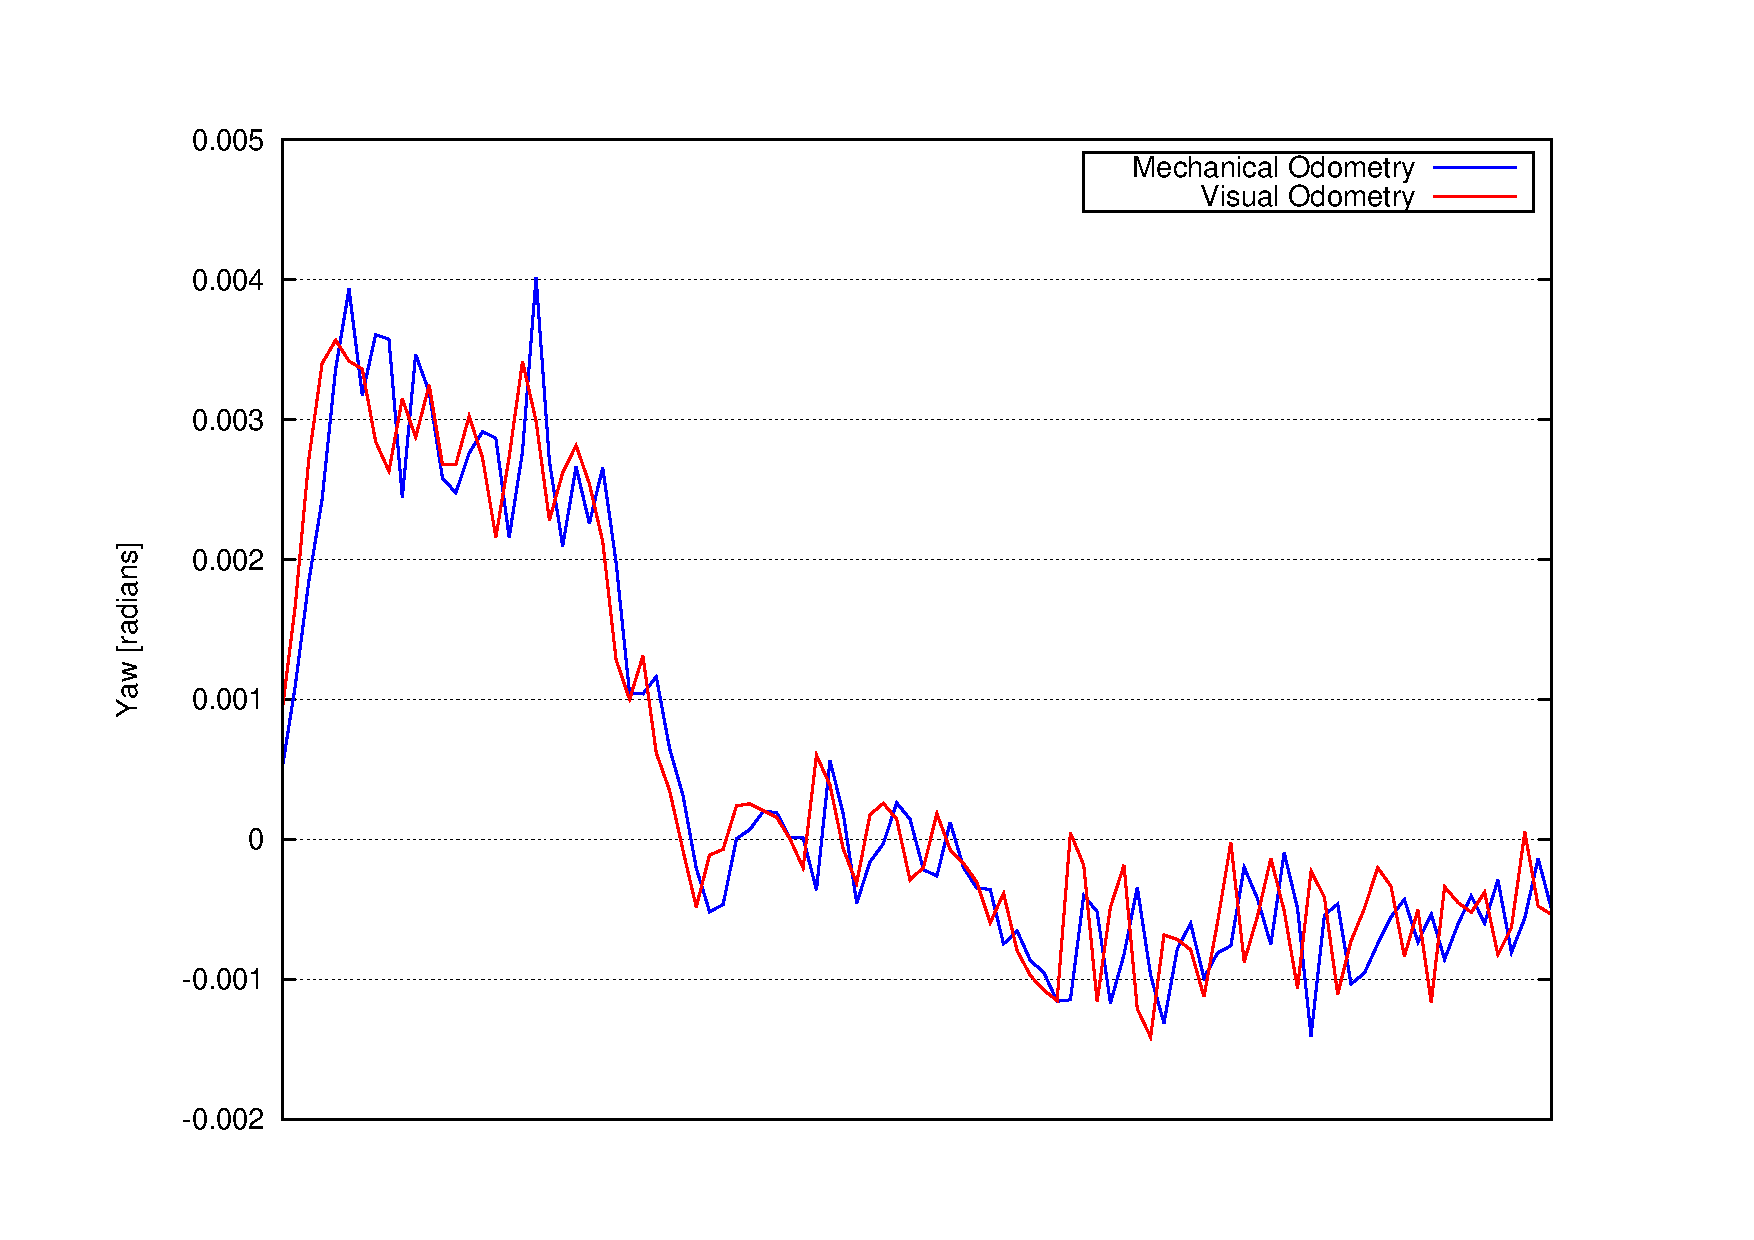
\includegraphics[trim=50 50 90 60, clip]{yaw}
  \caption{Comparison between the yaw values obtained through visual odometry compared to mechanical odometry.}\label{fig:cp05_ego_yaw}
\end{figure}

About the speed, shown in figure \ref{fig:cp05_ego_speed}, we observe that the shape of the obtained results are quite similar, but with a constant difference of about 0.5\,m/s between the results of both methods. We have concluded that the reason for that could be an error in the calibration for the cameras. As we are using visual odometry just for evaluation reasons, this bias in the speed is acceptable, as the speed difference between frames looks correct, as the similar shape of the curves suggests.

\begin{figure}[th]
  \centering
  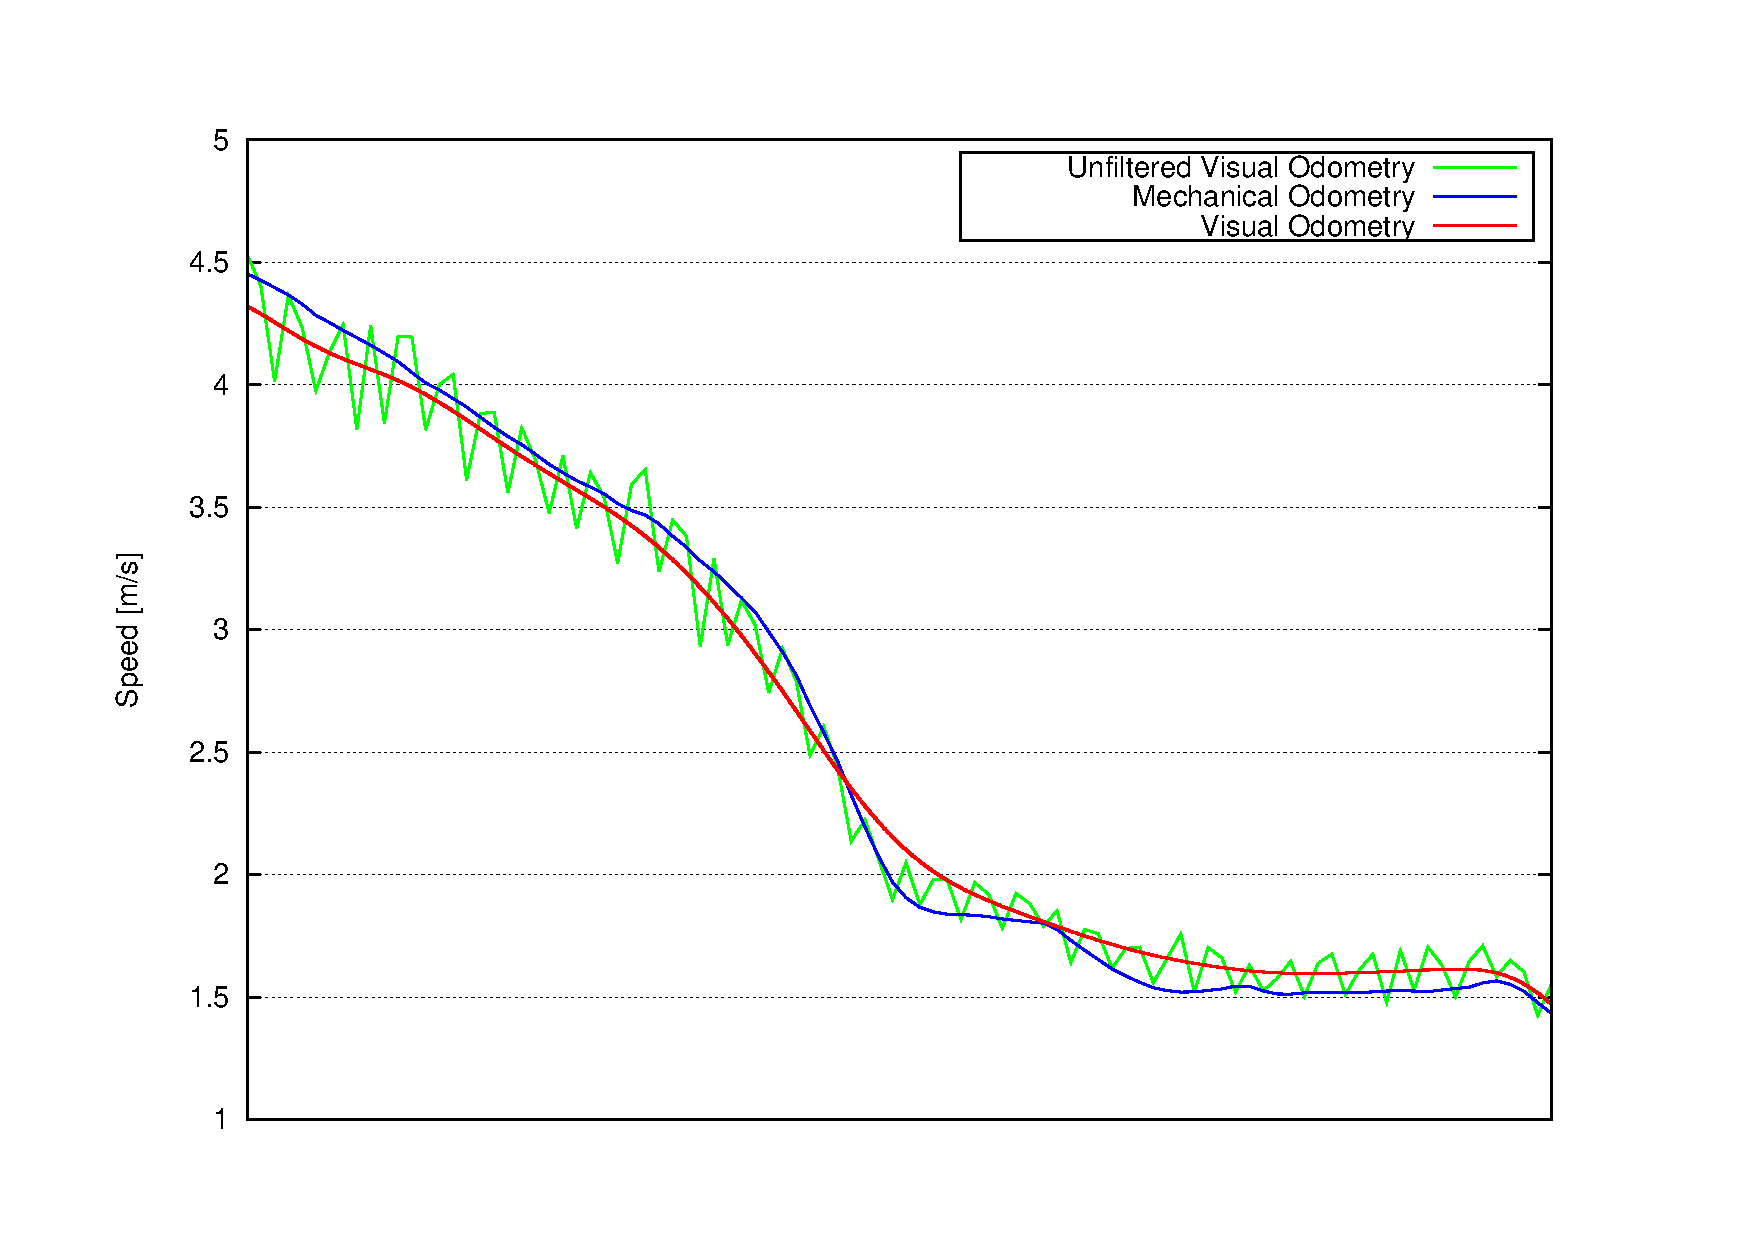
\includegraphics[trim=50 50 90 60, clip]{speed}
  \caption{Comparison between the speed values obtained through visual odometry compared to mechanical odometry.}\label{fig:cp05_ego_speed}
\end{figure}

After analyzing the results provided by these tests, we have concluded that results should be similar by using the visual and mechanical odometry.

\section{Detection}\label{ch:chapter05_02_03}
\todo{Si me sobra tiempo, intentar hacer un estudio más exhaustivo usando las imágenes de Daimler}

In this section, we want to compare our results with those obtained by our implementation of the method developed by \ref{danescu2012particle}, which is named as \emph{Cell based PF tracking}. For this purpose, we have used a base a dataset of stereo pairs for which we know the localization of the obstacles (\cite{geiger2013vision}). For each frame, once we have detected and segmented the obstacles, we reproject the obstacle back to the left image. Around this reprojected obstacle, we define a \ac{ROI} that represents the area covered by this obstacle. In the dataset used, there is information of bounding boxes around the obstacles (pedestrian, vehicles, etc...), that can be used as input for the computation of the \emph{true positives}, \emph{true negatives} and \emph{false negatives} using the standard intersection-over-union criterion (superior to 0.5). Unfortunately, we did not found any dataset that allow us to evaluate the segmentation limits quality (as we are using voxels, we can segment more accurately that with a simple cuboid detection, as discussed before), but we think that a solution like that described is fair enough to have an idea of the goodness of our method. 

With the computed \emph{true positives}, \emph{true negatives} and \emph{false negatives}, the \emph{recall}, \emph{precision}, \emph{$f_1$} measure and \emph{similarity} values are calculated using the same method described in \todoref{XXX-CEP,eval}. From these values, we obtained the curves shown at figure \ref{fig:cp05_detection_rate}, which relate each of theses values with the percentage of frames under this value. In this sense, the fastest the curve grows in the $y-axis$ while the $x-axis$ grows, the better.

The number of particles used for these tests is $1000$, as we decide after performing the tests described in the next section.

% Tasa de deteccion
\begin{figure*}[th]
        \centering
        \begin{subfigure}[b]{0.5\textwidth}
                \centering
                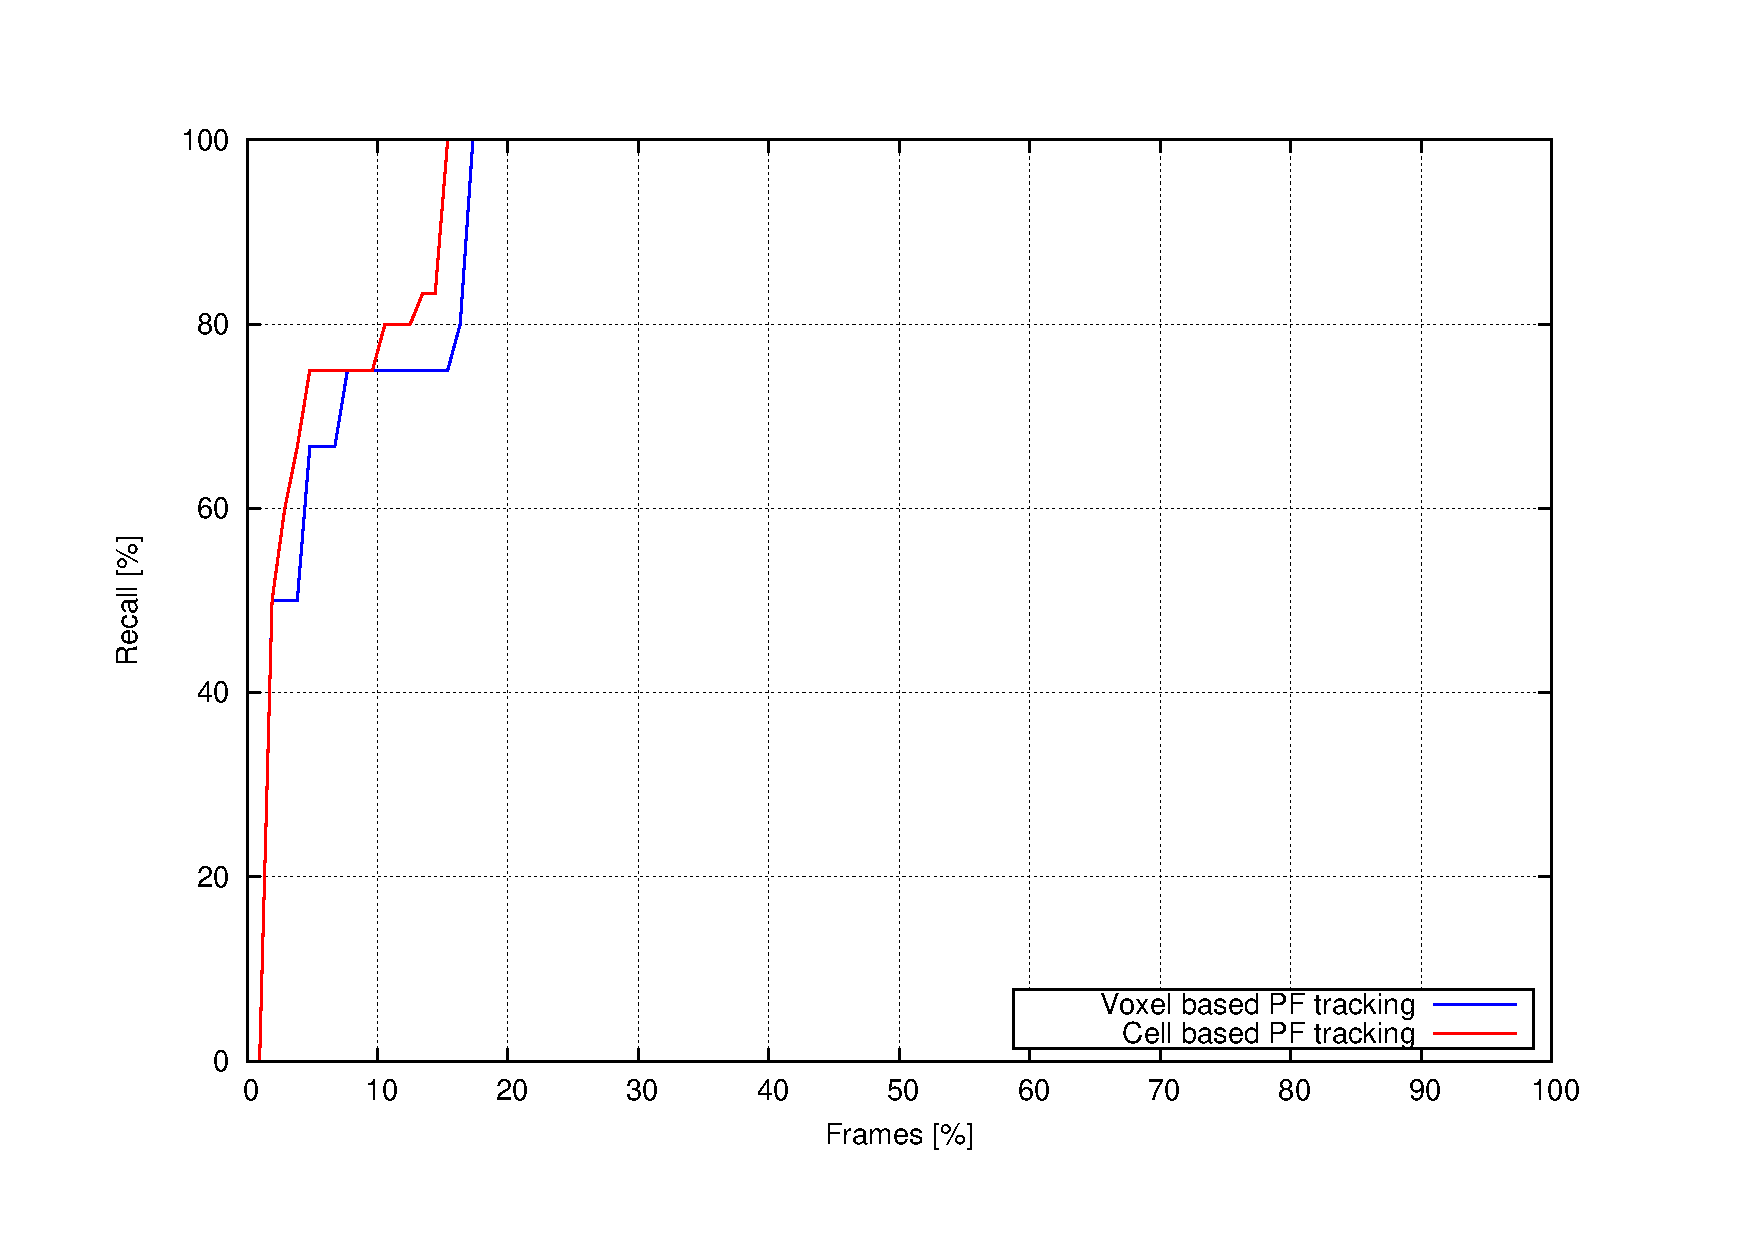
\includegraphics[width=\textwidth, trim=50 40 80 60,clip]{recall}\label{fig:cp05_recall}
                \caption{Recall}
                \label{fig:recallChart}
        \end{subfigure}%        
        ~ %add desired spacing between images, e. g. ~, \quad, \qquad etc.
          %(or a blank line to force the subfigure onto a new line)
        \begin{subfigure}[b]{0.5\textwidth}
                \centering
                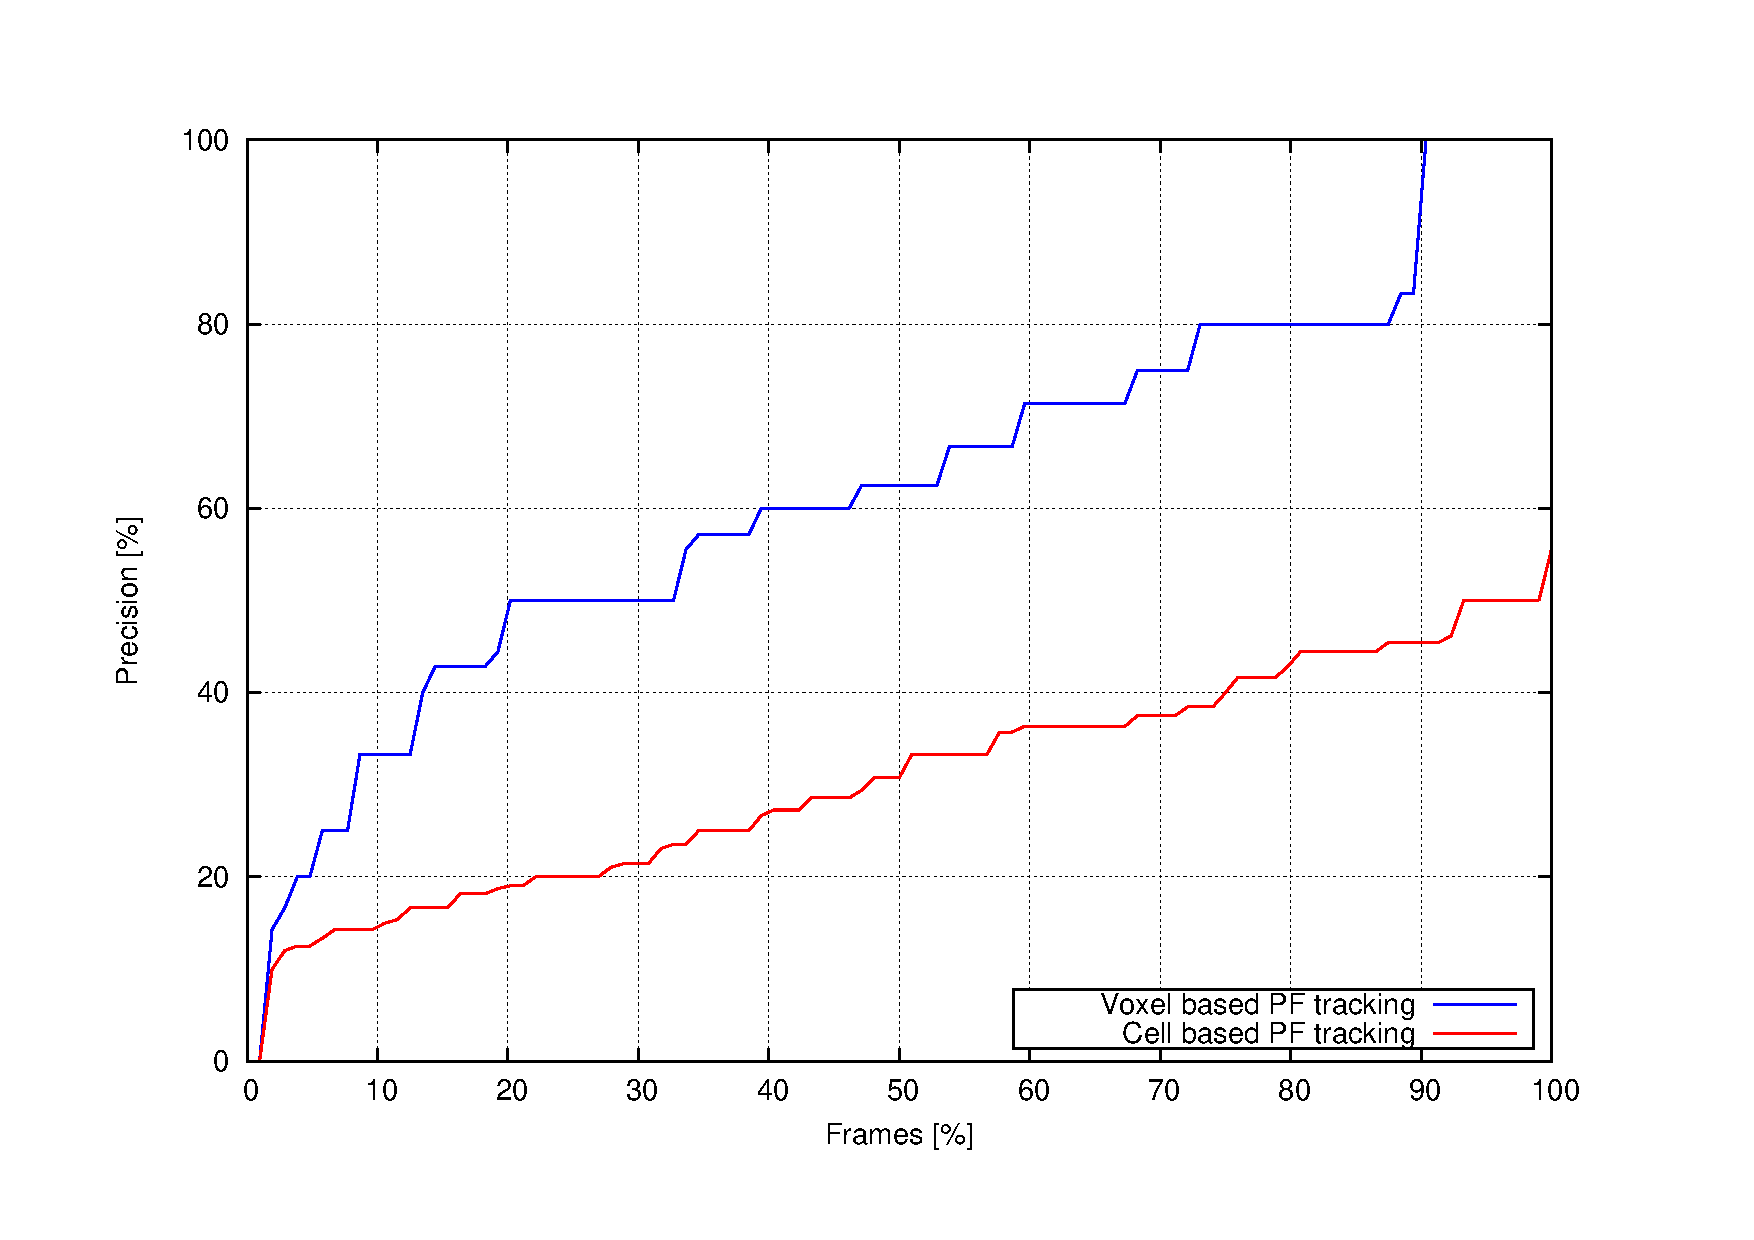
\includegraphics[width=\textwidth, trim=50 40 80 60,clip]{precision}\label{fig:cp05_precision}
                \caption{Precision}
                \label{fig:precisionChart}
        \end{subfigure}%
        
%         ~ %add desired spacing between images, e. g. ~, \quad, \qquad etc.
          %(or a blank line to force the subfigure onto a new line)
        \begin{subfigure}[b]{0.5\textwidth}
                \centering
                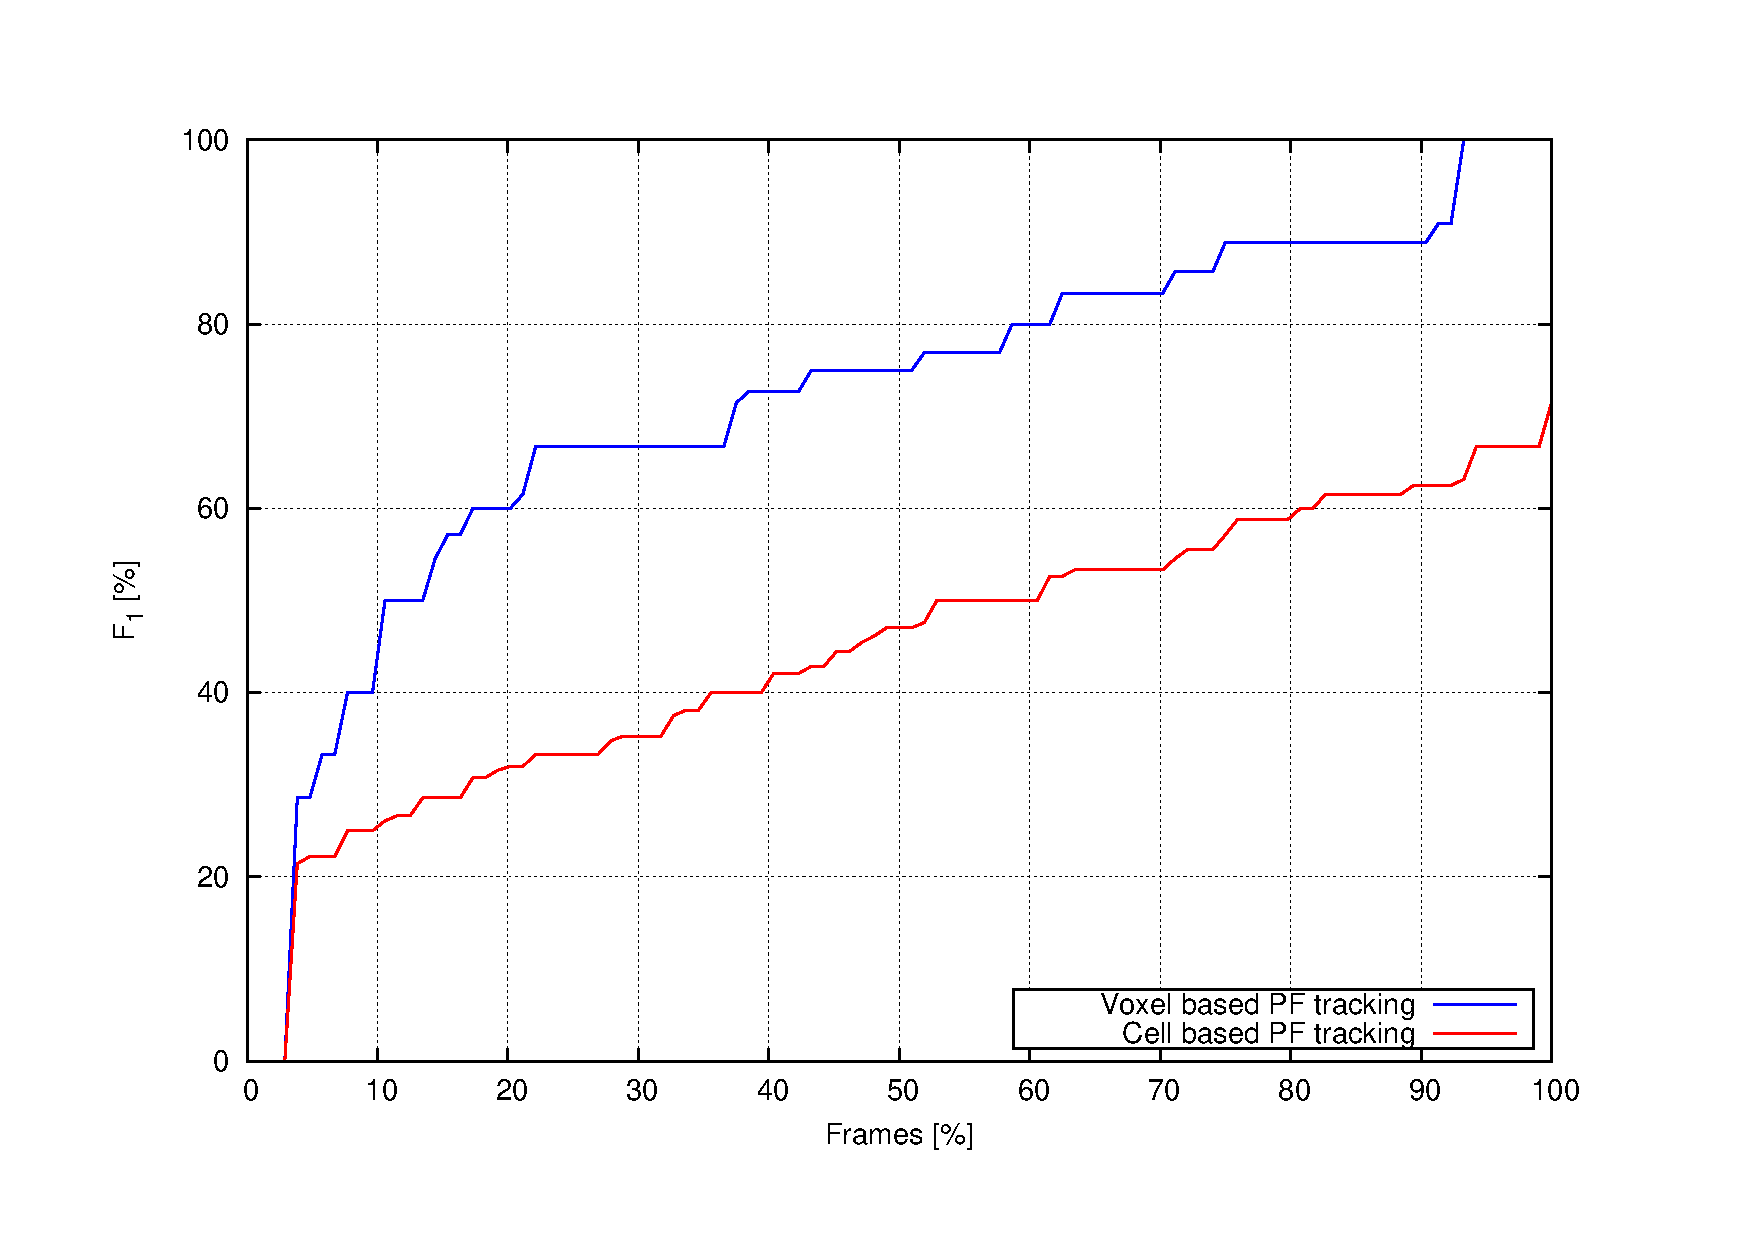
\includegraphics[width=\textwidth, trim=50 40 80 60,clip]{f1}\label{fig:cp05_f1}
                \caption{$F_1$}
                \label{fig:f1Chart}
        \end{subfigure}%
        ~ %add desired spacing between images, e. g. ~, \quad, \qquad etc.
          %(or a blank line to force the subfigure onto a new line)
        \begin{subfigure}[b]{0.5\textwidth}
                \centering
                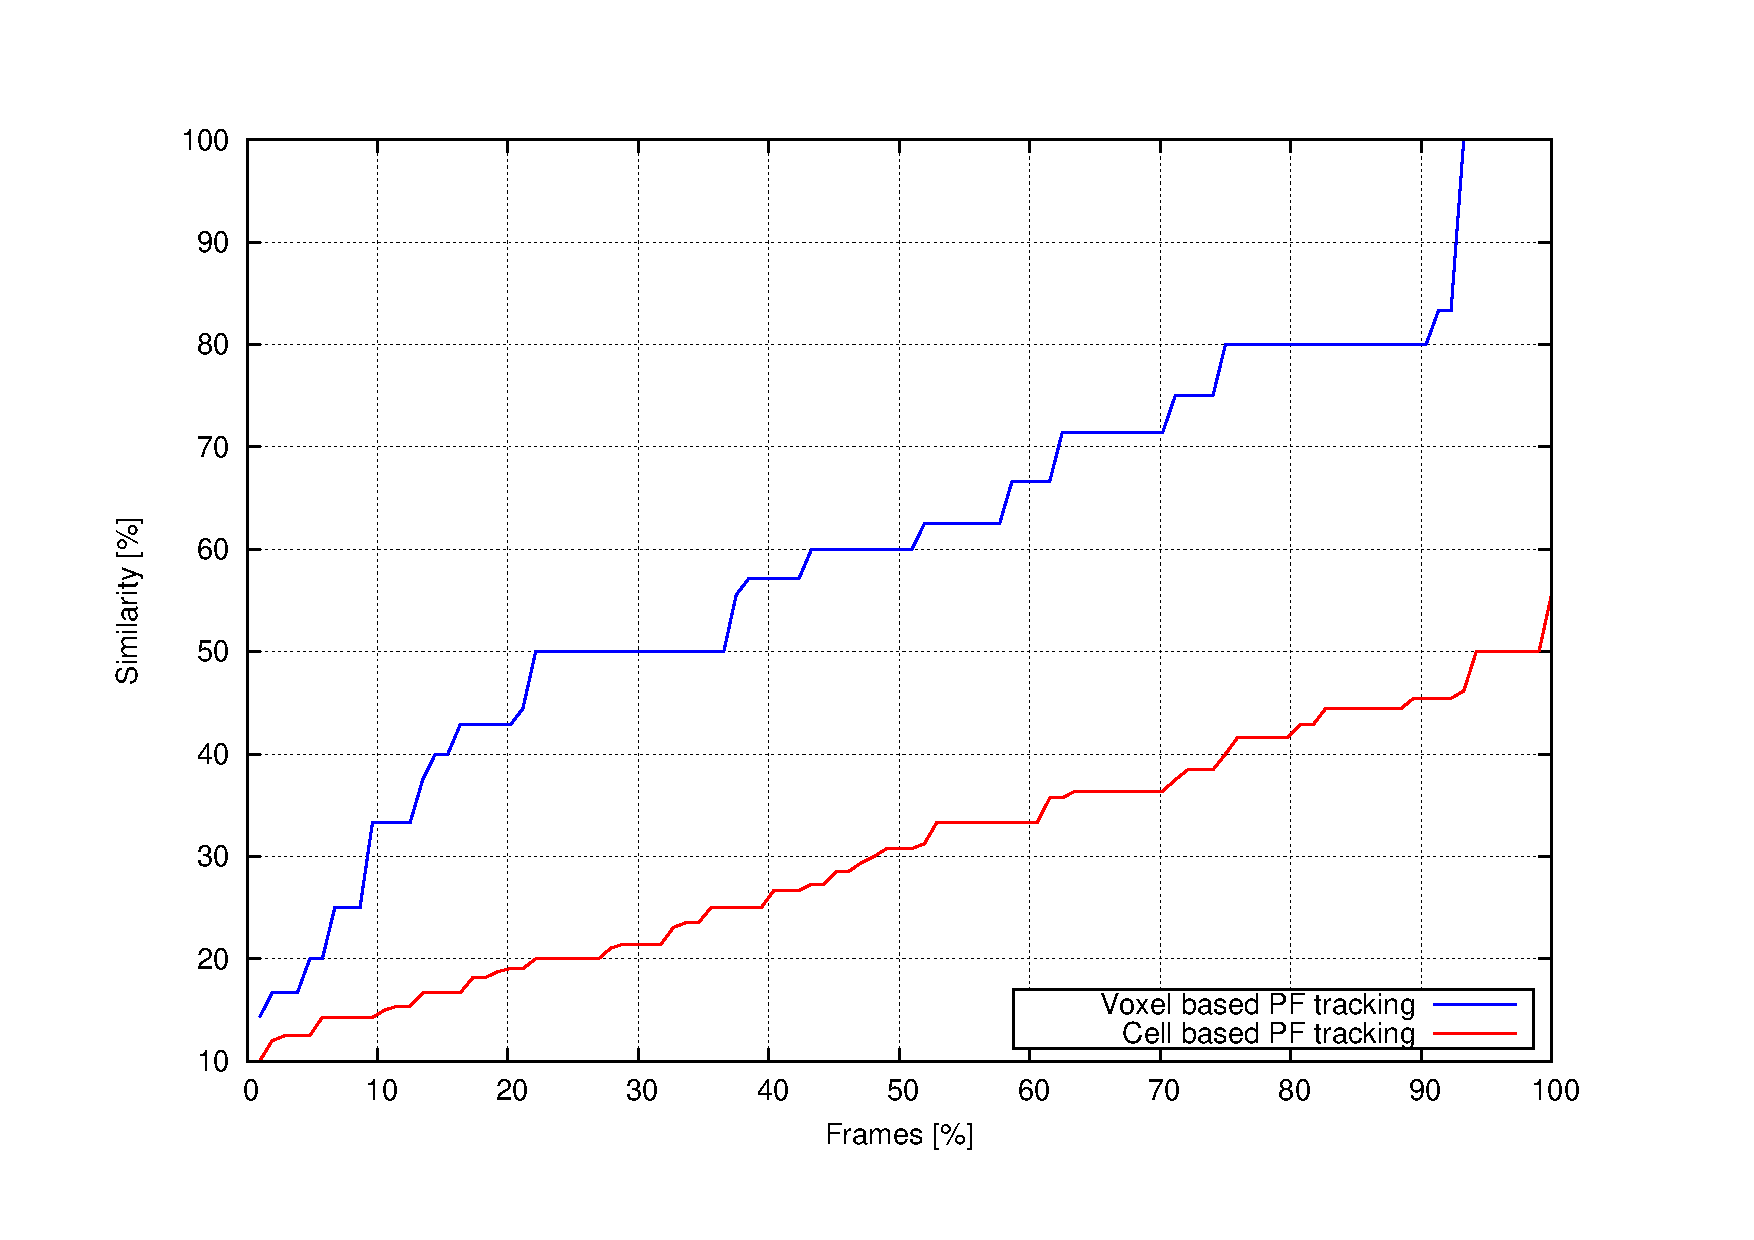
\includegraphics[width=\textwidth, trim=50 40 80 60,clip]{similarity}\label{fig:cp05_similarity}
                \caption{Similarity}
                \label{fig:similarityChart}
        \end{subfigure}
        \caption{Detection rate obtained by our method, compared with our implementation of the method of \cite{danescu2012particle}.}\label{fig:cp05_detection_rate}
\end{figure*}

In figure \ref{fig:recallChart}, we see that the behavior in both methods is pretty similar, despite the cell grid based method grows slightly faster. The number of frames with a good recall value is high, with about just less than a 15 percent of images with a recall value below 80\,\%. About precision, the difference is much more evident. Our method (\emph{Voxel based PF tracking}) grows faster than the other method does. The reason for which the cell grid is not so good is because experimentally we have noticed it tends to do over-segmentation, generating more obstacles than actually are. Regarding to our method, despite the results are better, they could be improved if we implemented a mechanism to detect static obstacles. As our method is particle-based, it is very difficult for a zero-speed particle to win, so objects always have a certain speed, even if they are static. A solution for that is rejecting those obstacles with a speed smaller than a parameterized threshold, but in this case we could eliminate obstacles that are actually going slow. Another safer option could be detecting the movement in the 2d images and mask those areas for which no movement is found.

The other two charts, representing the $F_1$ and $similarity$ values, allow knowing which is the method which represents a best compromise between the number of emph{true positives}, \emph{true negatives} and \emph{false negatives}. Again, best results with a noticeable difference are found for our method.

\section{Performance}\label{ch:chapter05_02_04}

One of the parameters that affect the most to the final results of the method is the number of particles. With a bigger number of particles, we will have a better representation of the probability distribution of the hypotheses, but the time needed for computation is increased. In this section, we describe the computation time oriented tests we performed in order to know the best number of particles configuration we could have, while knowing the real frequency at which our method is able to work.
In figure \ref{fig:cp05_time_vs_particles}, we show the results of these tests. There, a chart represents the computation time needed by the method for each frame of a given sequence. Each of the lines represent a certain number of particles.

% Relacion tiempo-particulas
\begin{figure}[th]
  \centering
  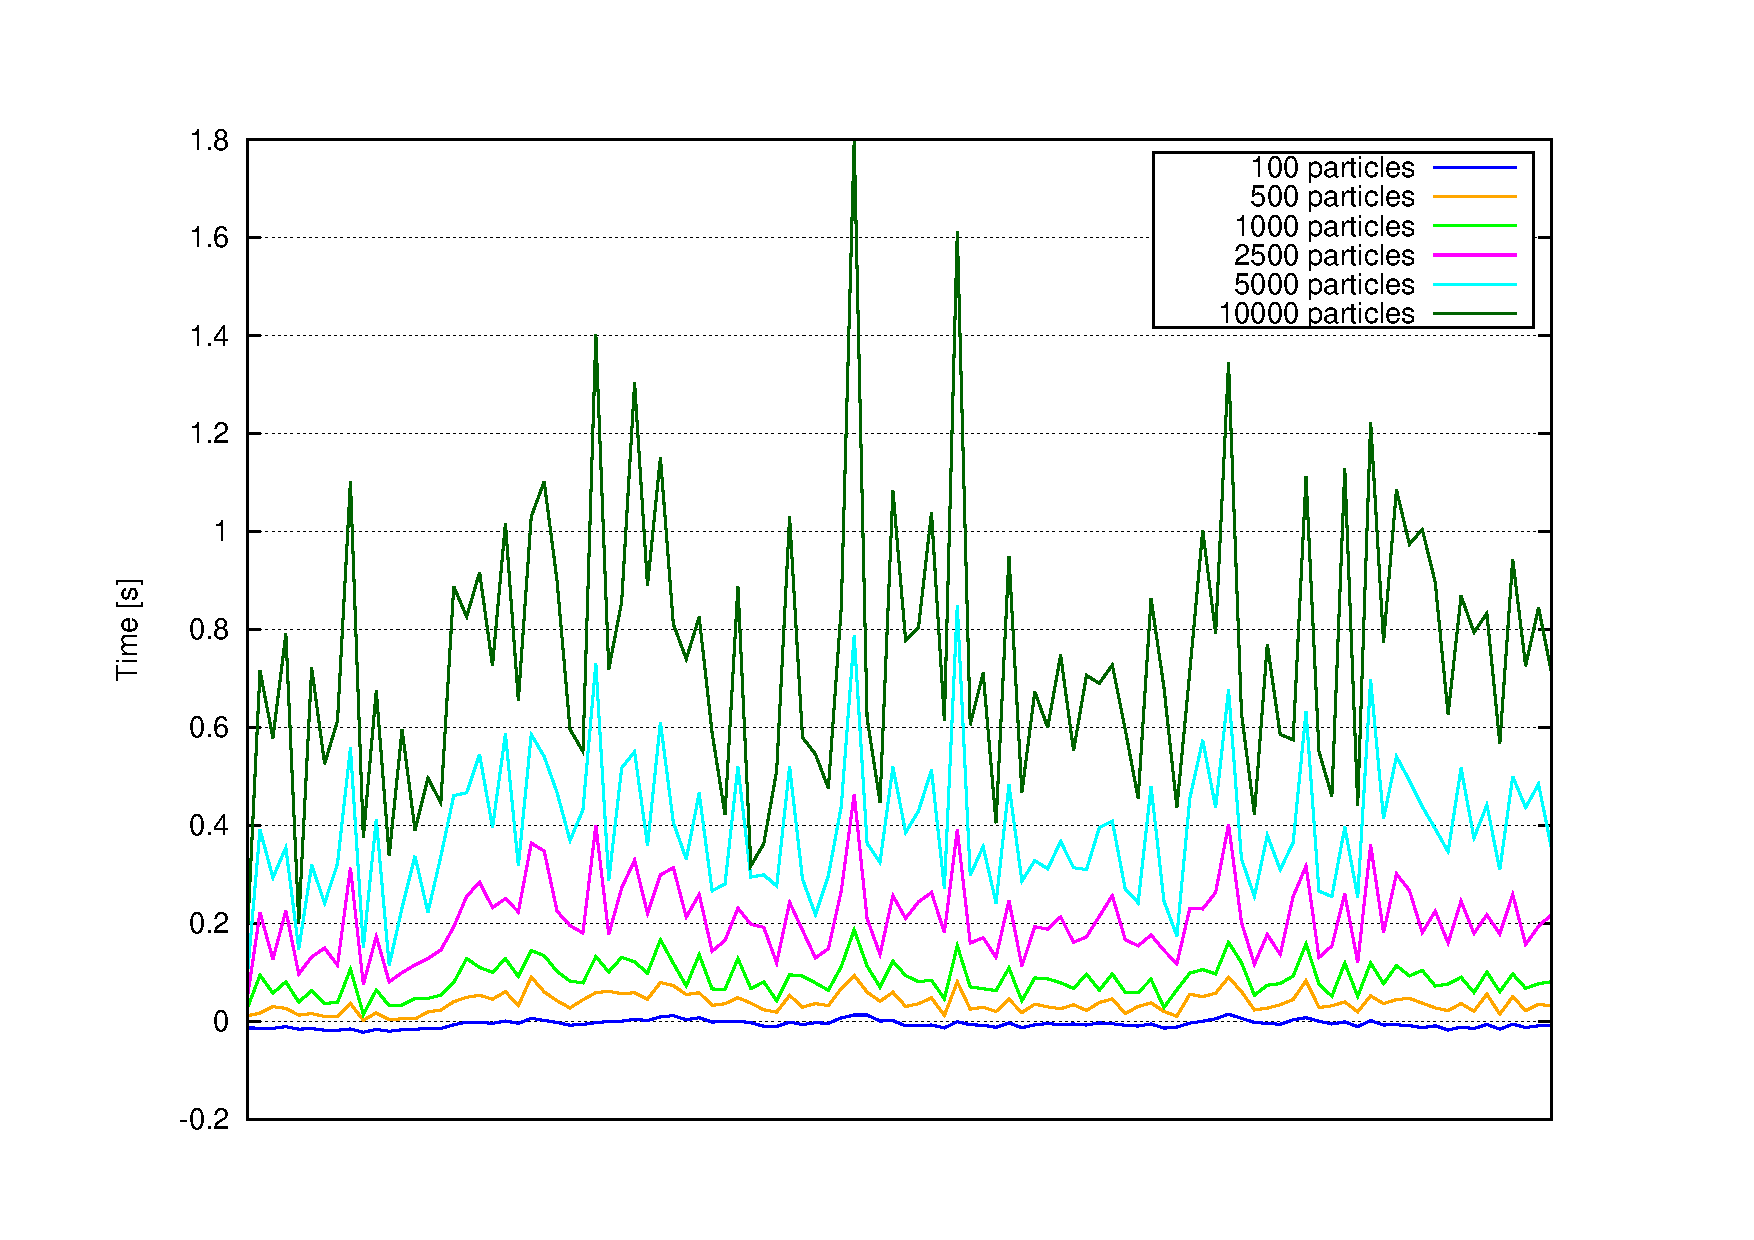
\includegraphics[trim=50 50 90 60, clip]{timesVsParticles}
  \caption{Comparison of the time needed for the each iteration when the number of particles increases.}\label{fig:cp05_time_vs_particles}
\end{figure}

As expected, the more particles we use, the more time the method needs to work. We considered that at least a maximal time of 0.2 s (5\,$Hz$) is reasonable for an application like this one. If we look at the chart, we can see that with 1000 particles, the maximal time reached is 0.2\,s. Also, for 2500 particles the average is around this value, but in this case, we are more interested in the maximal peak, that with this number of particle reaches more than 0.4\,s. Because of that, we finally decided to use 1000 particles in our tests, with the results previously shown. With this configuration, the method is able to work at an average between 6-7\,$Hz$ in an computer equipped with an Intel\textregistered\,i7 2.4\,$GHz$.
 
\section{Summary}\label{ch:chapter05_03}
 
In this chapter, we have introduced the method we used for the detection and tracking of obstacles in the environment of the car. This solution solves the main problems we had from the first approach we used for this purpose:
\begin{itemize}
 \item It is able to do the detection of obstacles and locate them in world coordinates, not just in image coordinates.
 \item It is able to work with real cameras.
 \item It is able to do that in real time.
 \item It is able to know the direction and speed of each obstacle.
\end{itemize}

The method comes with some advantages in comparison with other methods. Through the use of a particle filter based approach, the method is able to avoid complex probabilities-related calculations that can be simplified through the use of this tool. It is also able to work in three-dimensions without increasing the complexity, thanks to the use of a voxel grid. This allows also a more specific knowledge of the obstacle, which is not limited just to the more external boundaries of the obstacle through the use of cuboids. Finally, the implementation is quite modular, allowing to use as input any kind of point cloud, as no color information is used; and fast, being able to work at 6-7\,$Hz$.

In the future, we plan to do further research in order to improve the results given by the method. Some ideas are related to the use of color ( despite it would affect to the modularity of our system) as using more information should improve the output. We also think that using a polar voxel grid instead of a cartesian one would improve some results. Also, it would be a good idea to use a Kalman filter in order to track the detected obstacles, so we would know not just their position and current speed, but also their movement along the frames. Finally, we could take advantage of the big amount of operations that are done individually for each voxel and do a parallelized implementation that allows improving the algorithm frequency a little bit more or using a bigger number of particles.

In the next chapters, we will introduce the way in which paths are calculated, both in the sense of allowing the vehicle to reach the desired position but also in the sense that it should be able to avoid the obstacles detected using the method described in this chapter.
 
 
 
 